\chapter{Audio Frequency Scaling methods}\label{ch:scaling_methods}
\section{Introduction}
The human hearing system detects
acoustic vibrations and translates 
those vibrations into sounds.
The detectable range of frequencies by the human ear
is referred to as audio or sonic. This range
spans over approximately \(20\;kHz\),
starting at \(20\;Hz\) to about \(20\;kHz\)
\cite{hearthres}.

As a result of aging, the hearing system's dynamic range 
as to the detectable bandwidth decreases,
and by middle-age are set at about
\(20\;Hz\) to  \(14\;KHz\)\cite{Wiley2008ChangesIH}.
That is, the maximum hearable frequency
declines with age.

The human ear's ability to distinguish 
between two different frequencies 
is not symmetric. 
For example, the spectral distance between two 
different frequencies in one distinct region does 
not equal the spectral distance 
between two additional frequencies in other regions.
Due to that asymmetry, the conventional linear 
spectral mapping is impractical for
speech analysis applications.
Thus, a different spectral mapping 
based on a different scaling system
that mimics the human hearing as possible
is applied instead as an alternative.

\section{Mel-Scaling}
The Mel-scaling method 
is a suggested solution to mapping 
standard audio frequencies to perceived frequencies.
The basic idea that lies underneath it is that for
different pitches we assign varying bandwidth,
such that they are equal in distance
from each other, as rated by listeners.
The reference point has been chosen to be 
\(1000\;Hz = 1000\;Mels\).

Mel-scale was first described in \cite{Volkmann} by Stevens and Volkmann,
where the authors presented different curves for Mel-scaling.

Two common tables were composed
according to the Mel-scaling curves. One table by 
Beranek in 1949 \cite{beranek1988acoustical} 
and the second by Umesh et al. in 1999 \cite{fitmelscale}.

The most popular equation that models the Mel-scale
is typically referenced as
the "Logarithm based Mel scale"\cite{o1987speech}:
\begin{equation}\label{eq:mel_1}
    Mel = \ln \left( 1 + \frac{f}{700} \right) \cdot \frac{1000}{\ln(1+\frac{1000}{700})} 
\end{equation}

Equation\;[\ref{eq:mel_1}] can be simplified as follows:
\begin{align}
    Mel & = 1127 \ln \left( 1 + \frac{f}{700} \right) \nonumber \\
    Mel & = 2595 \log_{10}\left( 1 + \frac{f}{700} \right)
\end{align}

\bigskip
\bigskip
\bigskip
\bigskip
\bigskip
\bigskip
Then, the reverse equation, converting Mels back to Hz,
can be written as:
\begin{align}
    f[Hz] & = 700 \left( 10^{\frac{Mel}{2595}} -1  \right)
\end{align}

% \subsection{Logarithm based Mel scale}
% The most popular equation that models the Mel-scale
% is given by \cite{o1987speech}:
% \begin{equation}
%     Mel = \ln \left( 1 + \frac{f}{700} \right) \cdot \frac{1000}{\ln(1+\frac{1000}{700})} 
% \end{equation}
% This can be simplified as follows:
% \begin{align}
%     Mel & = 1127 \ln \left( 1 + \frac{f}{700} \right) \nonumber \\
%     Mel & = 2595 \log_{10}\left( 1 + \frac{f}{700} \right)
% \end{align}
% Then, the reverse equation, converting Mels back to Hz,
% can be written as:
% \begin{align}
%     f[Hz] & = 700 \left( 10^{\frac{Mel}{2595}} -1  \right)
% \end{align}
% These modeling equations became de-facto the default way to
% map audio frequencies to Mels.

\subsection{Mel-scale approximations}
Computing a logarithm for hardware devices, 
whether it is the natural logarithm or any other base, 
is not very straightforward.
For example, this kind of computation might require special
techniques or long LUTs (look-up tables),
which are extraordinarily resource hungry.

Instead, other approximations that do not involve
trigonometric or logarithms, but only
simple arithmetic structures can be applied.
By doing so, we benefit from low resource
utilization while maintaining high accuracy.

Multiple approximation methods were studied in \cite{fitmelscale}.
Two approximations are the most prominent for target HW devices.
\begin{align}
    \label{eq:melapproxa} Mel & = a + b \cdot f \\ 
    Mel & = \frac{f}{a \cdot f + b} \label{eq:melapproxb}
\end{align}

Where \(a\), \(b\) in Equation \ref{eq:melapproxa} are defined as follows:
\begin{align}
    a & = \begin{cases}
        127.7   &,\;f \leq 1000 \\
        1322    &,\;f > 1000
    \end{cases} \nonumber \\
    b & = \begin{cases}
        0.9     &,\;f \leq 1000 \\
        0.19    &,\;f > 1000
    \end{cases}
\end{align}

while in Equation \ref{eq:melapproxb} \(a\), \(b\) are:
\begin{align}
    a & = \begin{cases}
        0.000244   &,\;f \leq 1000 \\
        0.0004    &,\;f > 1000
    \end{cases} \nonumber \\
    b & = \begin{cases}
        0.741   &,\;f \leq 1000 \\
        0.603   &,\;f > 1000
    \end{cases}
\end{align}

\begin{figure}[H]
    \centering
    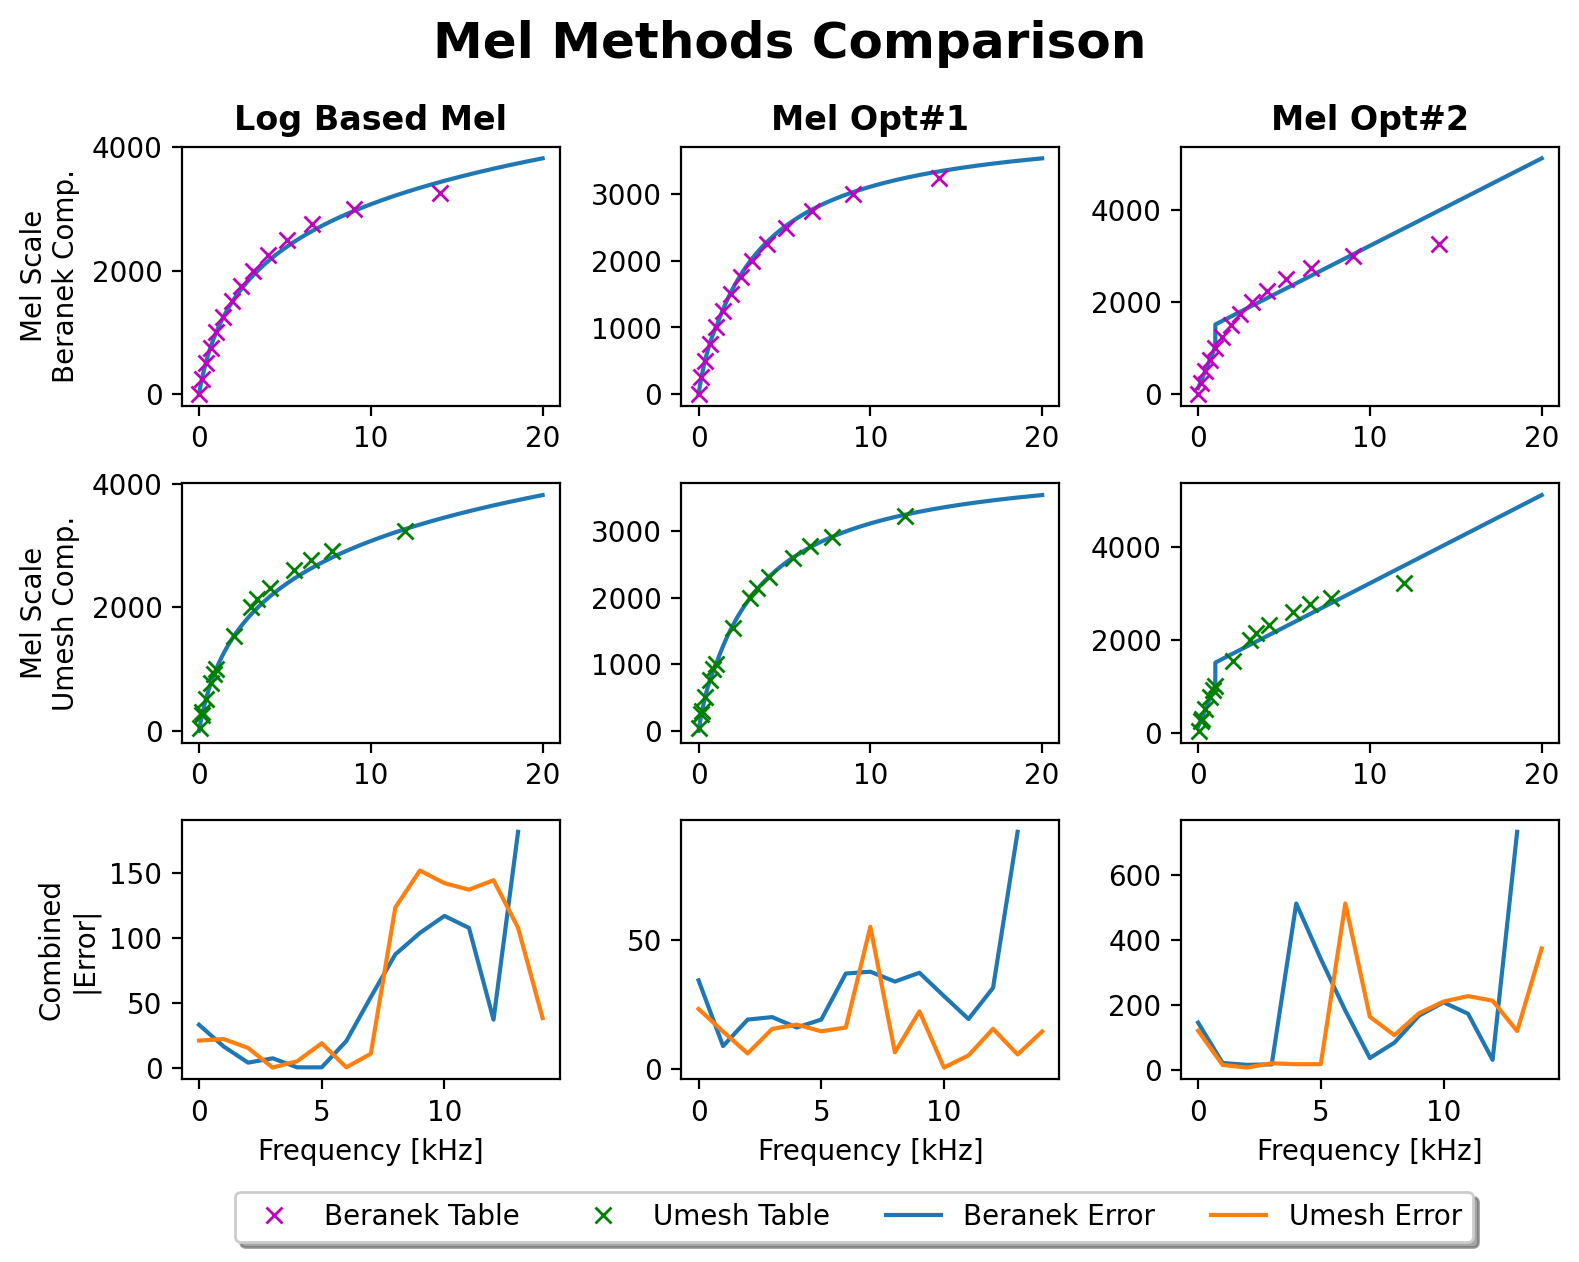
\includegraphics[width=\linewidth]{Scaling/images/mel_methods_comp}
    \caption{Mel-scale comparisons with Beranek \& Umesh tables}\label{fig:mel_methods_comp}
\end{figure}

Figure \ref{fig:mel_methods_comp} has comparisons of three different 
Mel-scale implementations with Beranek \& Umesh tables.
The first column, Log Based Mel, represents
O'Shaugnessy's famous log-based Mel modeling.
The Mel option \#1, and Mel option \#2 columns 
follow the suggested approximations
given in Equations \ref{eq:melapproxa} 
and \ref{eq:melapproxb}, respectively.

From the last row of graphs, we can deduce that the approximation
in Equation~\ref{eq:melapproxb} 
is the closest along with the range of audio frequencies
to the tables provided by Beranek \& Umesh.
On the other hand, the more simplified approximation 
in Equation~\ref{eq:melapproxa} seems 
to yield the highest errors.

\begin{figure}[H]
    \centering
    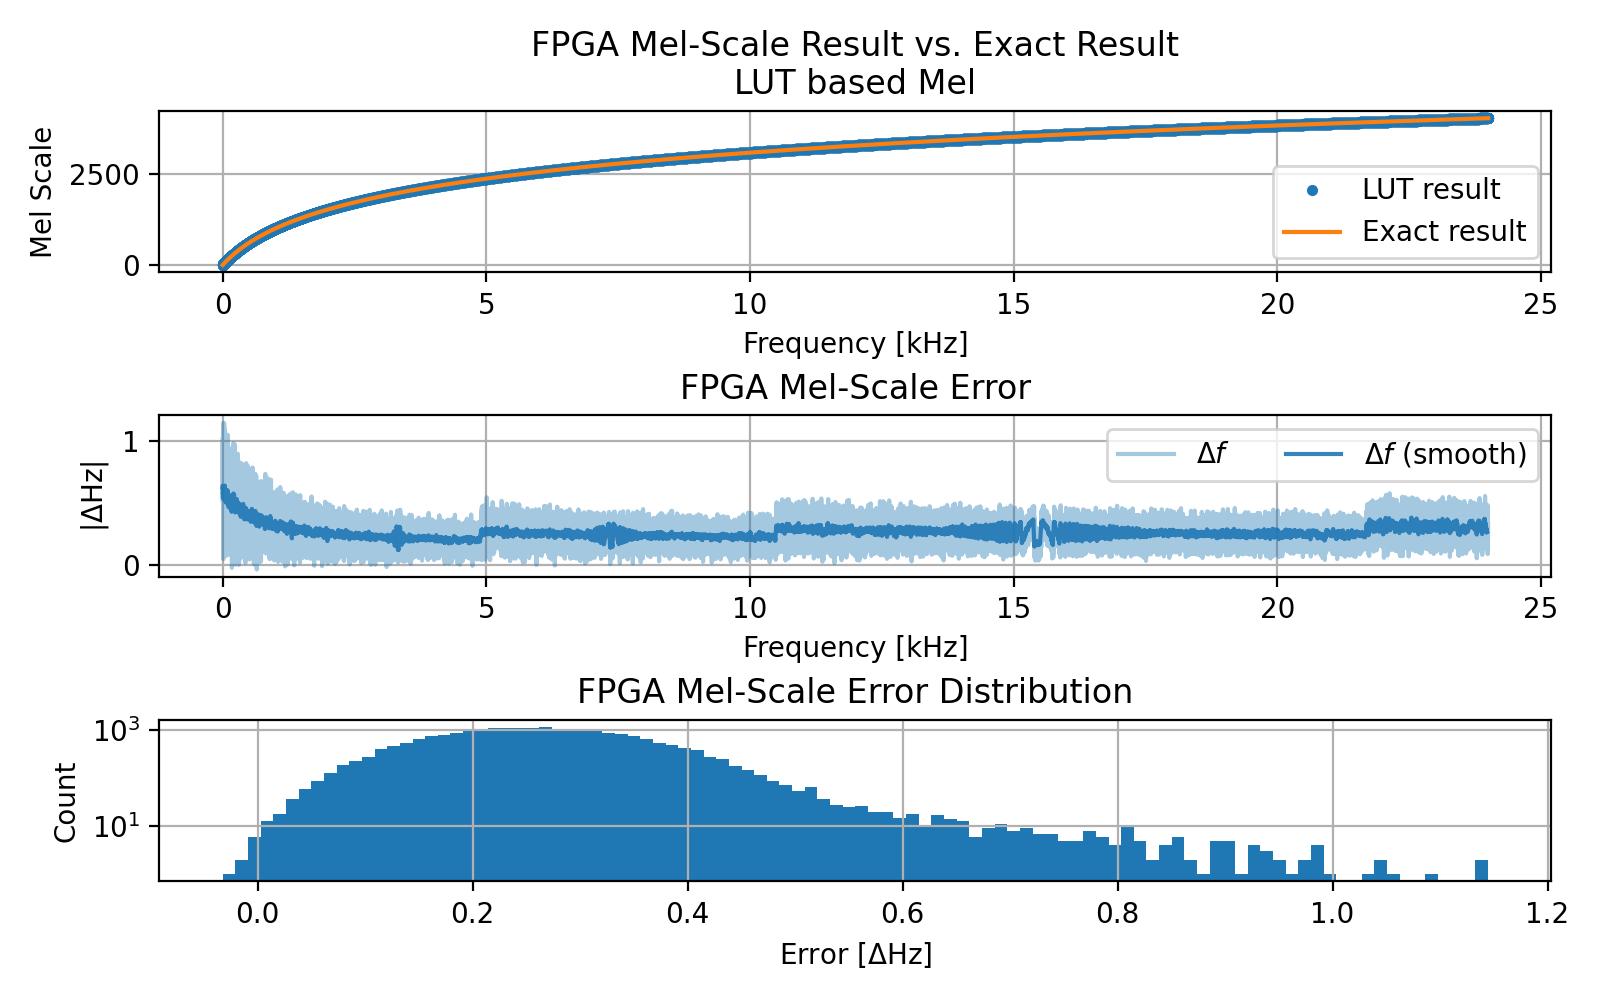
\includegraphics[width=\linewidth]{Scaling/images/mel_lut}
    \caption{LUT based Mel FPGA implementation results}\label{fig:mel_lut}
\end{figure}

\begin{figure}[H]
    \centering
    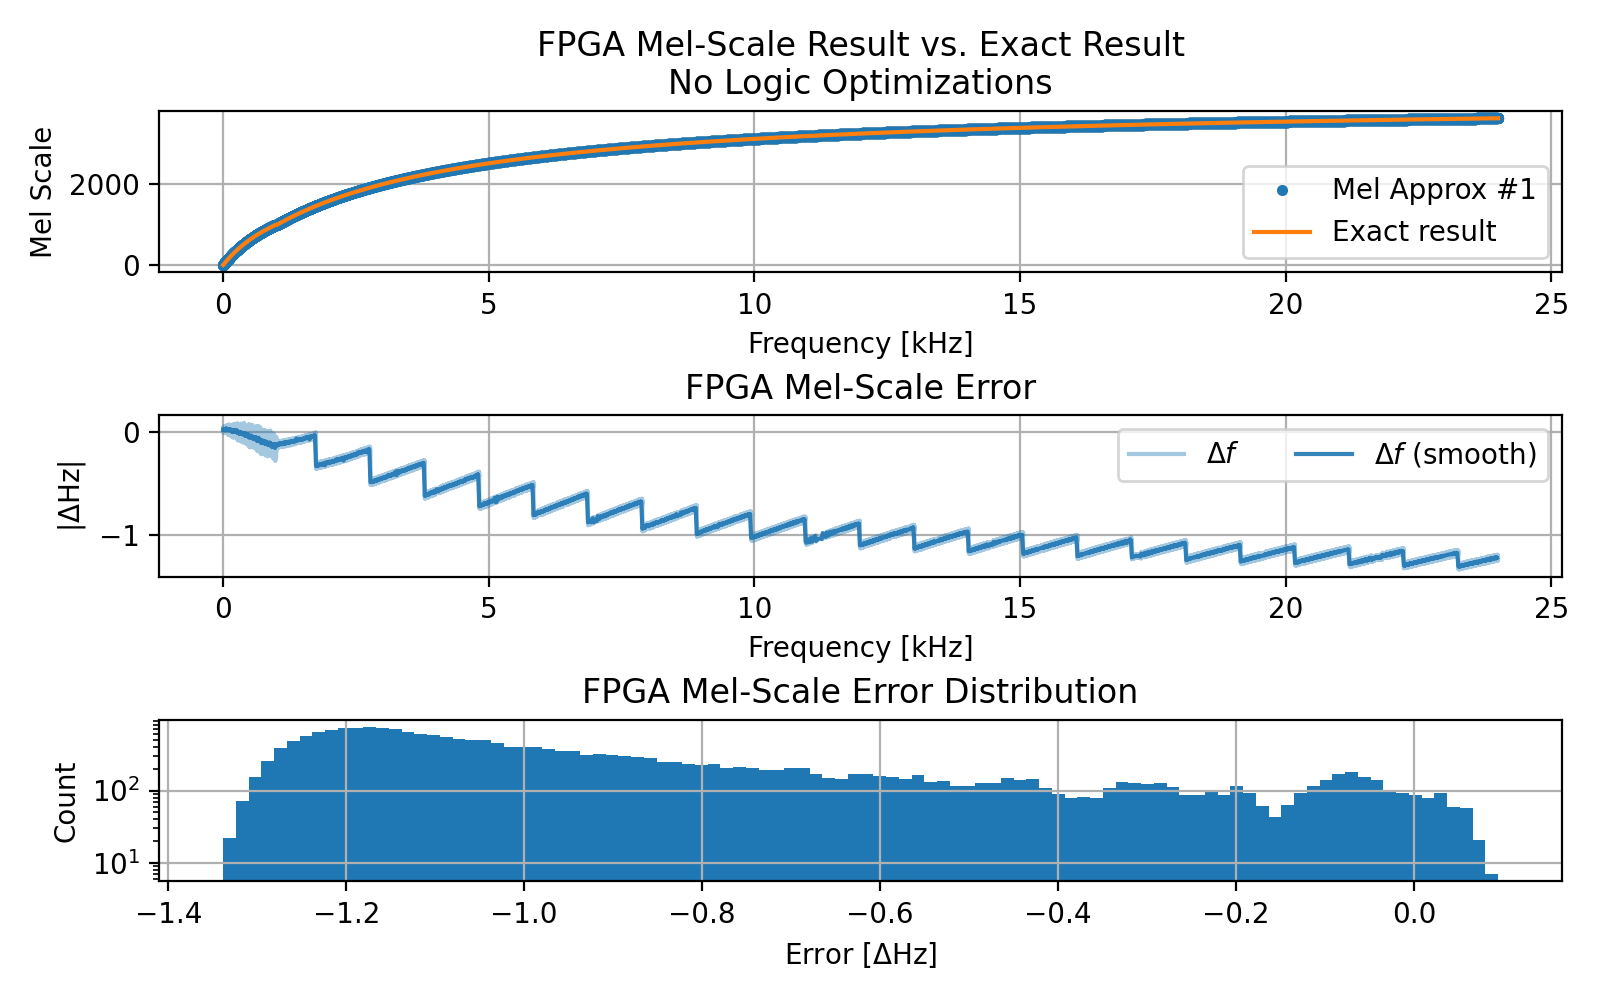
\includegraphics[width=\linewidth]{Scaling/images/mel_approx_no_opt}
    \caption{Mel approx. \#1 FPGA implementation results}\label{fig:mel_approx_no_opt}
\end{figure}

Figures \ref{fig:mel_lut}, \ref{fig:mel_approx_no_opt} 
present the results of FPGA implementations
of O'Shaugnessy's log-based Mel and Mel approximation \#1.
Nonetheless, a high precision quantization, U32.22 was chosen
for the Mel approximation, where 
the shifting error received is higher when compared 
to the conventional Log Mel scaling implementation.
Although this error shift is compensated 
just by selecting the approximation method, 
the straightforward approach 
turned out to be the non-optimized solution 
in terms of HW resources and power consumption,
which utilized four times higher wattage on top of \(25 - 30 \%\) 
additional resources.

Instead, two optimization workarounds were tested.
The first is the multiplication of the \(a, b\) coefficients
in Equation~\ref{eq:melapproxb} by 1000. 
The second optimization is reorganizing the equation
and storing the result in a sufficient precision structure in memory
for the fractional part but lower resolution for the integer part.  
These optimizations lead to a reduction in the 
required number of bits for the fractional part.
As a result, both the frequency shifting error 
and the overall resource utilization are greatly improved.

Yet, the split in frequency bands results in two multiplied sets
of coefficients for each band calculation.
Therefore, choosing a more generalized set 
of coefficients for the entire audio band can help 
in the reduction of redundant LUTs and other combinational logic, 
such as selectors and multi-bus multiplexer cells.

Selection of \(a=0.24,\;b=0.741\), showed better results
as can be seen in Figure \ref{fig:mel_approx_logic_opt_generic}.
The accuracy estimation for the non-generic implementation
is shown in Figure\;\ref{fig:mel_approx_logic_opt}.

\begin{figure}[H]
    \centering
    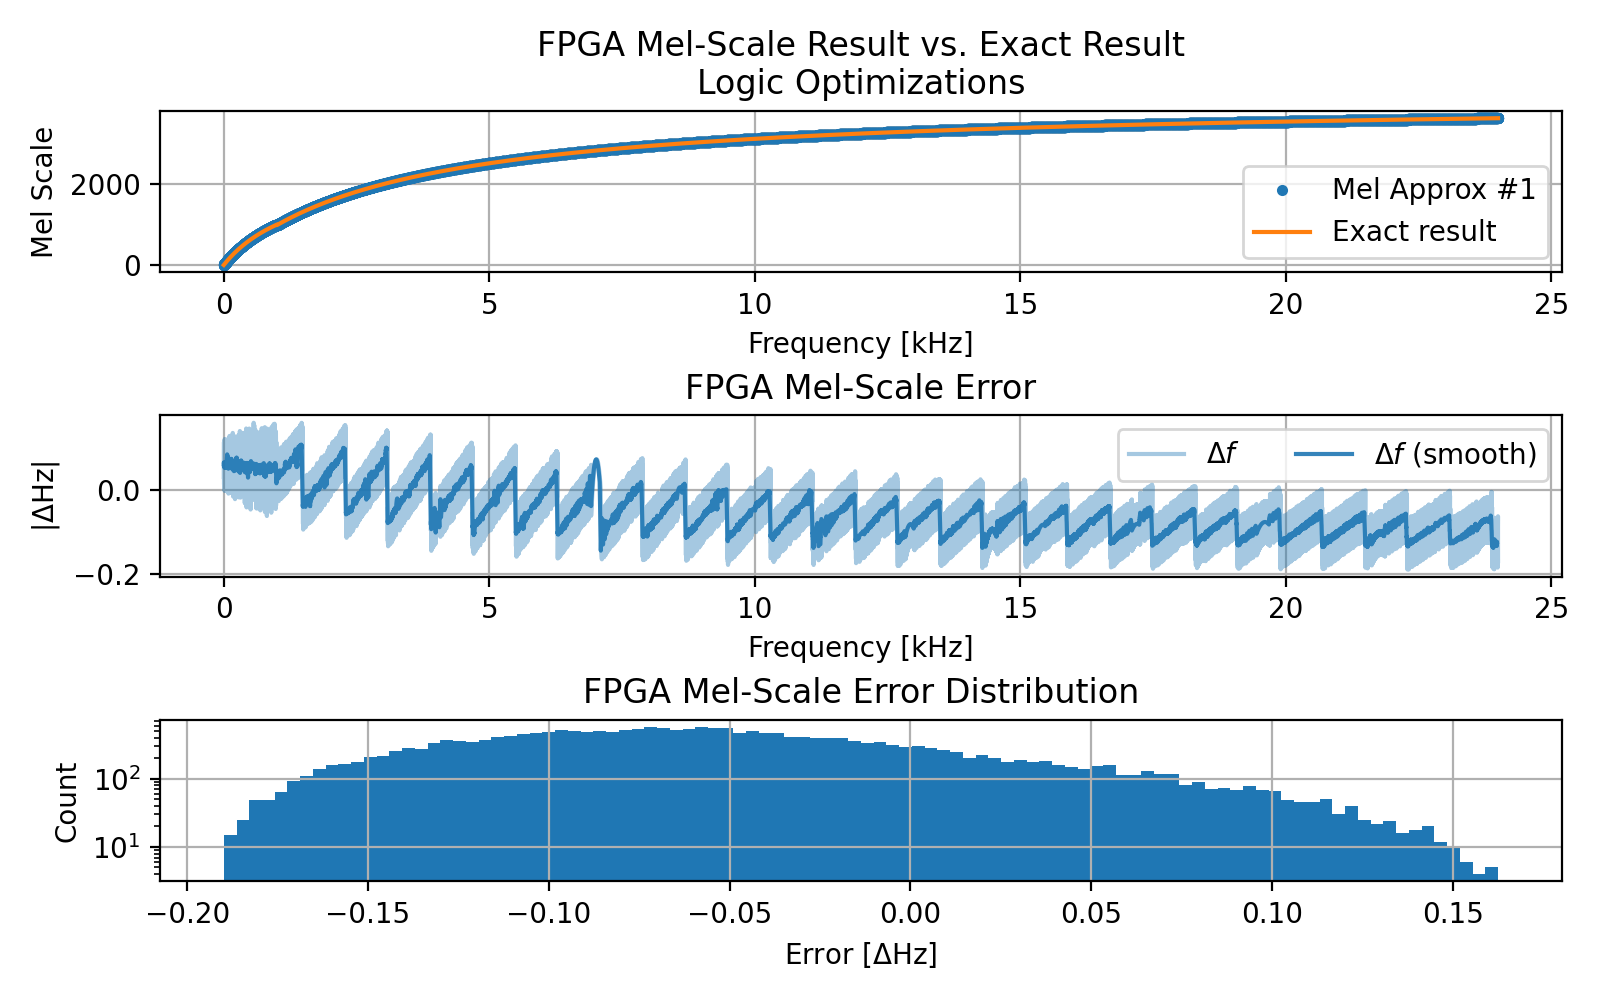
\includegraphics[width=\linewidth]{Scaling/images/mel_approx_logic_opt}
    \caption{Mel approx. \#1 \underline{optimized} FPGA implementation results}\label{fig:mel_approx_logic_opt}
\end{figure}


\begin{figure}[H]
    \centering
    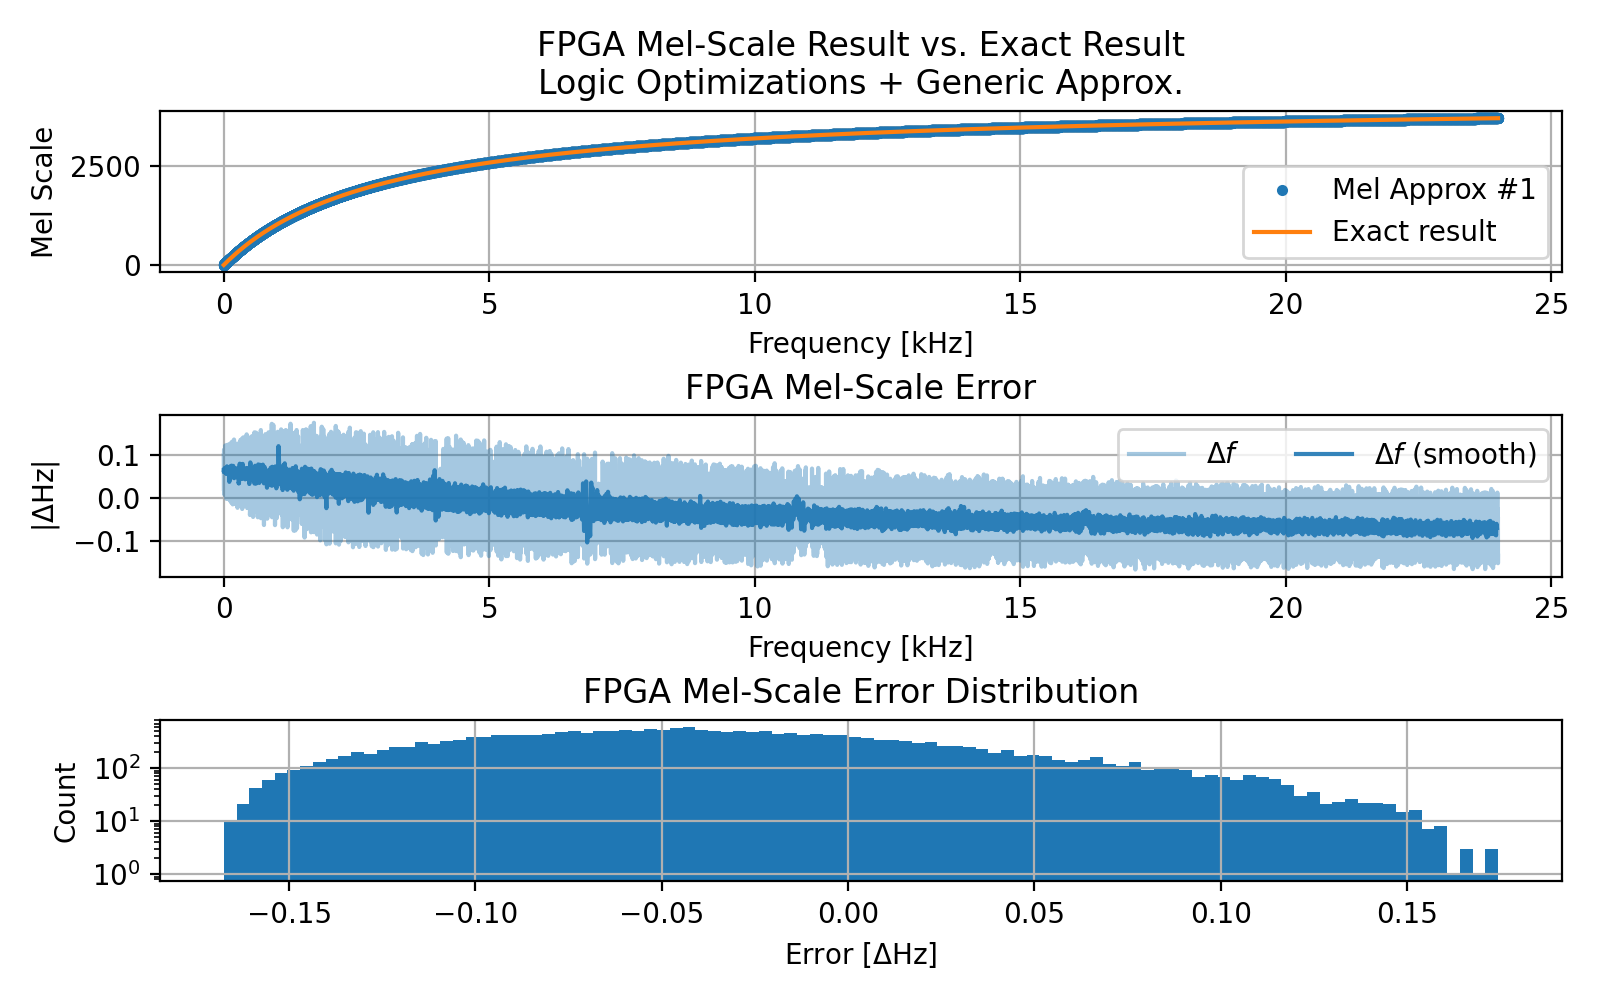
\includegraphics[width=\linewidth]{Scaling/images/mel_approx_logic_opt_generic}
    \caption{Mel approx. \#1 \underline{optimized, generic} FPGA implementation results}\label{fig:mel_approx_logic_opt_generic}
\end{figure}


\begin{table}[H]
    % for more info see: https://www.overleaf.com/learn/latex/tables
    % \centering
    \hspace*{-1.8cm}
    \arrayrulecolor{mtblborder}
\begin{tabular}{ !{\color{mtblborder}\vrule}l!{\color{mtblborder}\vrule}rcccc| } 
    \hline

    \hline
    \rowcolor{mtblcaption} \color{white}\bf{Algorithm} 
    & \color{white}\bf{Latency \([ns]\)}  
    & \color{white}\bf{Quant.} 
    & \color{white}\bf{Max Err. \([\Delta Hz]\)}
    & \color{white}\bf{Mean Err.}
    & \color{white}\bf{Std Err.} \\
    \hline

    \hline
    \rowcolor{mtbl} Log LUT Mel   & \(14\) (3 C.C) & U16/4 & 1.146 & 0.268 & 0.106 \\
    \hline
    
    \hline
    \rowcolor{wtbl} Mel \#1   & \(9\) (2 C.C) &  U32/22  & 1.338 & -0.873 & -0.359 \\
    \hline
    
    \hline
    \rowcolor{mtbl} Mel \#1 Opt      & \(9\) (2 C.C) &  U16/4  & 0.190 & -0.053 & 0.065 \\
    \hline

    \hline
    \rowcolor{wtbl} Mel \#1 Generic     & \(9\) (2 C.C) &  U16/4  & \color{gtblcaption}0.174 & \color{gtblcaption}-0.035 & \color{gtblcaption}0.061 \\
    \hline

    \hline
\end{tabular}
\arrayrulecolor{black}
\caption{Mel-Approx, log-based Mel performance comparison}
\label{tbl:mel_scale_performance}
\end{table}


\begin{table}[H]
    % for more info see: https://www.overleaf.com/learn/latex/tables
    \centering
    \arrayrulecolor{ytblborder}
\begin{tabular}{ !{\color{ytblborder}\vrule}l!{\color{ytblborder}\vrule}rrrrr| } 
    \hline

    \hline
    \rowcolor{ytblcaption} \color{white}\bf{Algorithm} 
    & \color{white}\bf{FF} 
    & \color{white}\bf{LUT} 
    & \color{white}\bf{DSP} 
    & \color{white}\bf{LUTRAM} 
    & \color{white}\bf{BRAM} \\
    % & \color{white}\bf{ORM} 
    % & \color{white}\bf{Clean} \\
    \hline

    \hline
    \rowcolor{ytbl} Log LUT Mel   & 82(0.04\%) & 276(0.23\%) & 1(<1\%) & 10(0.02\%) & 1.5(1.04\%)  \\
    \hline
    
    \hline
    \rowcolor{wtbl} Mel \#1     & 47(0.02\%) & 530(0.45\%) & 1(<1\%) & 0(0\%)  & 0(0\%)    \\
    \hline
    
    \hline
    \rowcolor{ytbl} Mel \#1 Opt      & 47(0.02\%) & 271(0.23\%) & 1(<1\%) & 0(0\%)  & 0(0\%)    \\
    \hline

    \hline
    \rowcolor{wtbl} Mel \#1 Generic     & \color{gtblcaption}47(0.02\%) & \color{gtblcaption}269(0.19\%) & \color{gtblcaption}1(<1\%) & \color{gtblcaption}0(0\%)  & \color{gtblcaption}0(0\%)    \\
    \hline

    \hline
\end{tabular}
\arrayrulecolor{black}
\caption{Mel scaling methods resource utilization table}
\label{tbl:mel_resource_util}
\end{table}



\begin{table}[H]
    % for more info see: https://www.overleaf.com/learn/latex/tables
    \centering
    \arrayrulecolor{gtblborder}
\begin{tabular}{ |l|cccc| } 
    \hline

    \hline
    \rowcolor{gtblcaption} \color{white}\bf{Parameter} 
    & \color{white}\bf{Log LUT Mel} 
    & \color{white}\bf{Mel \#1} 
    & \color{white}\bf{Mel \#1 Opt} 
    & \color{white}\bf{Mel \#1 Generic} \\
    \hline\hline
    \rowcolor{wtbl}\multicolumn{5}{|c|}{\bf{Dynamic Power [W]}}\\
    \hline
    \rowcolor{gtbl} Signals                 & 4.947 & 5.221 & 3.011 & 2.916  \\
    \hline
    
    \hline
    \rowcolor{wtbl} Logic                   & 6.50 & 6.792 & 3.751 & 3.070  \\
    \hline

    \hline
    \rowcolor{gtbl} DSP                     & 0.014 & 0.013 & 0.014  & 0.014 \\
    \hline
    
    \hline
    \rowcolor{wtbl} I/O                     & 18.236 & 26.263 & 7.207  & 6.378 \\
    \hline
    
    \hline
    \rowcolor{gtbl} \(\mathbf{P_{dynmic}}\) & \textbf{29.697} & \textbf{38.290} & \textbf{13.983}  & \textbf{\colorbox{Goldenrod!70}{\color{MidnightBlue}12.379}} \\
    \hline

    % \hline
    % \rowcolor{gtbl} Bark Scale      & 56(0.02\%) & 218(\%) & 1(<1\%)   \\
    % % \cline{2-8}
    % % \multirow{-2}{*}{\cellcolor{ytbl}\#1(5)}   & 14.03/17.78 & 27.06 & 13.73 & - & - & - & 7.72 \\ 
    \hline\hline
    \rowcolor{wtbl}\multicolumn{5}{|c|}{\bf{Static Power [W]}}   \\
    \hline

    \hline
    \rowcolor{gtbl} PL Static               & 2.364 & 2.466 & 0.499  & 0.499 \\
    \hline
    
    \hline
    \rowcolor{wtbl} PS Static               & 0.068 & 0.071 & 0.020 & 0.018  \\
    \hline

    \hline
    \rowcolor{gtbl} \(\mathbf{P_{static}}\) & \textbf{2.432} & \textbf{2.537} & \textbf{0.519} & \textbf{\colorbox{Goldenrod!70}{\color{MidnightBlue}0.517}}  \\
    \hline

    \hline\hline
    \rowcolor{wtbl}\multicolumn{5}{|c|}{\bf{Total Power [W]}}   \\
    \hline

    \hline
    \rowcolor{gtbl} \(\mathbf{P_{total}}\)  & \textbf{32.13} & \textbf{40.827} & \textbf{14.502} & \textbf{\colorbox{Goldenrod!70}{\color{MidnightBlue}12.896}}  \\
    \hline
\end{tabular}
\arrayrulecolor{black}
\caption{Mel-Approx, log-based Mel, Bark Scale Power consumption}
\label{tbl:mel_scale_pwr_tbl}
\end{table}

The LUT implementation makes use of a \(log_{2}\) look-up table.
However, an additional step is 
needed for the natural logarithm or other log bases. 
Since the logarithm bases are constant, 
the LUT result is divided by the \(log_{2}\) of the base,
whether it be the natural base or base ten.
This logarithm bases 
convention is described in Equation\;\ref{eq:log_base_conv}.
\begin{align}\label{eq:log_base_conv}
    \log_{b}(a)  & = \frac{\log_{x}(a)}{\log_{x}(b)}
\end{align}


Table\;\ref{tbl:mel_scale_performance} summarizes
the performance comparison between the different Mel scaling
implementation approaches. 

The HW setup is for the PYNQ-Z1 development board.
Hence, the results are unique to that specific 
HW device and probably change for other 
FPGA devices and development boards.

Latencies were simulated with Xilinx Vivado Suite
for an operating clock frequency of \(225\;MHz\).
In this operating condition, no timing violations were reported.

Tables\;\ref{tbl:mel_resource_util} and \ref{tbl:mel_scale_pwr_tbl}
show the synthesis and implementation results 
plus the power estimation reports. 
These reports were taken from the Xilinx Vivado Suite application.

\section{Bark-Scaling}
Another scaling method is the Bark scale which is based on
the same principle of retaining perceptual distances.
The Bark scale is divided into critical 
bands corresponding to the critical hearing bands in humans. 
Each band has a bandwidth similar 
to the psychoacoustic band of the corresponding 
``filter'' in the human hearing system 
and is ranked with a unique number.

\subsection{Bark Critical Bands}
Like the Mel scale, several equations were proposed to model best
the Bark scale and its critical bands.

The first method was introduced in \cite{1908630}.
A proposed approximation to the Bark scaling is described in 
\cite{TraunmullerScale}; this paper also introduces the 
correction of the band boundaries to ensure more 
correctness with the original Bark scaling.

Four different equations were proposed to model
the Bark scale.

The first by Zwicker is well described in\cite{1908630} and
is given by the following equation:
\begin{align}% Zwicker Eq
    Bark & = \tan^{-1}\left\{ 0.00073f \right\} + 3.5 \tan^{-1}\left\{ 
            \left( \frac{f}{7500} \right)^{2}
        \right\}
\end{align}

Zwicker's bark scale and it's corresponding critical bands
are shown in Figure \ref{fig:Zwicker_bark}
\begin{figure}[H]
    \centering
    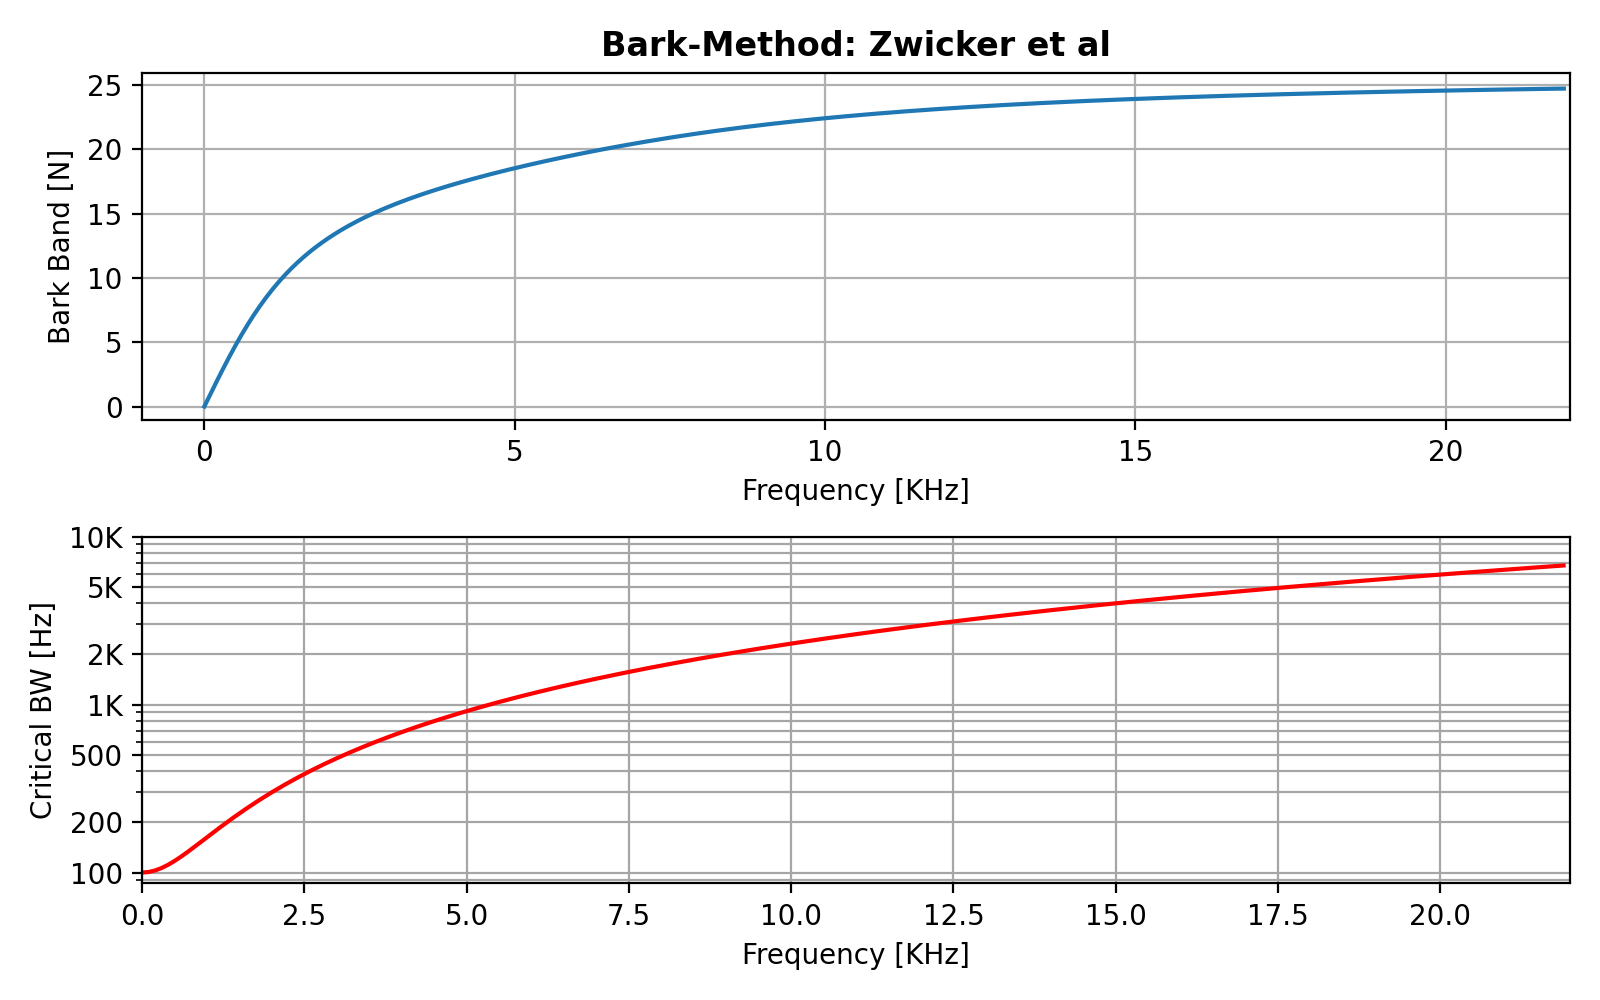
\includegraphics[width=0.75\linewidth]{Experiments/images/Zwicker}
    \caption{Zwicker's bark scale and critical bands}\label{fig:Zwicker_bark}
\end{figure}

Another proposed equation by Traunmuller \cite{TraunmullerScale} is:
\begin{align}\label{eq:traunmuller_no_fix}% Traunmuller Eq + Correction
    Bark & = \frac{26.81f}{1960 + f} - 0.53
\end{align}

Traunmuller's bark scale and it's corresponding critical bands
are shown in Figure \ref{fig:Traunmuller_nofix}
\begin{figure}[H]
    \centering
    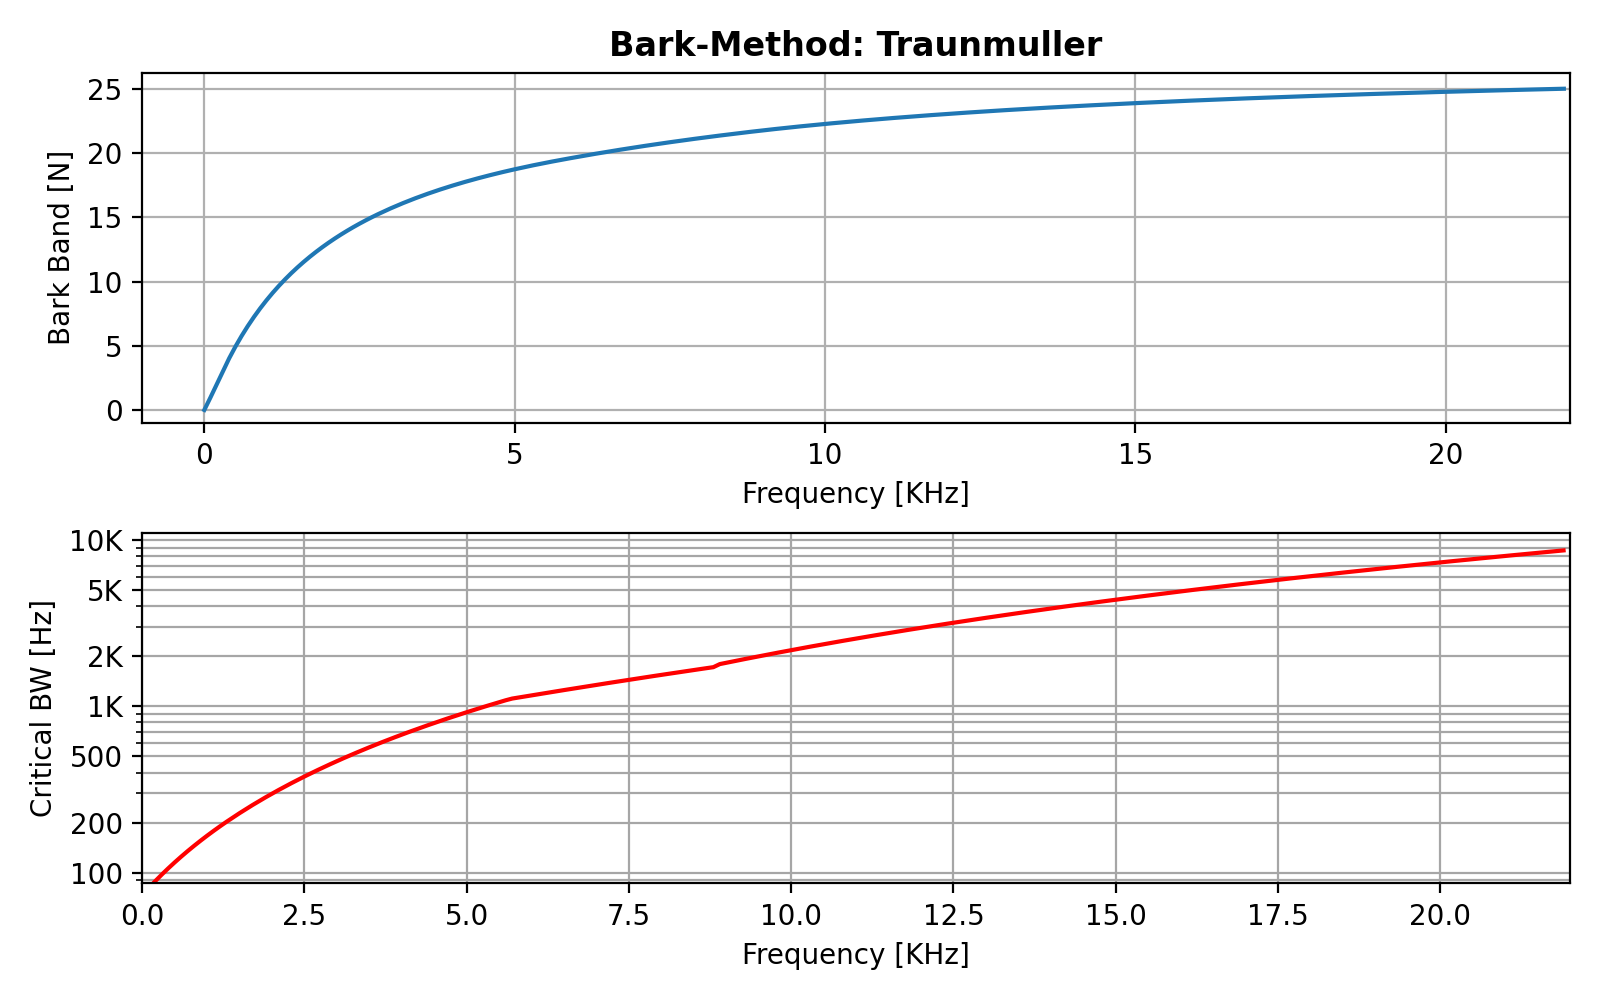
\includegraphics[width=0.75\linewidth]{Experiments/images/Traunmuller_nofix}
    \caption{Traunmuller's original bark scale and critical bands}\label{fig:Traunmuller_nofix}
\end{figure}

Denoting Traunmuller's original
Bark scale given in Equation \ref{eq:traunmuller_no_fix} as \(Bark'\),
the fixed form for Traunmuller's Bark equation is:
\begin{align}
    Bark & = \begin{cases}
        0.3 + 0.85\cdot \left( Bark' \right) 
        &,\;Bark' < 2 \\
        Bark' + 0.22\cdot \left( Bark' - 20.1 \right) 
        &,\;Bark' > 20.1
    \end{cases}
\end{align}

Traunmiller's fixed bark scale and its corresponding critical bands
are shown in Figure \ref{fig:Traunmuller_fix}
\begin{figure}[H]
    \centering
    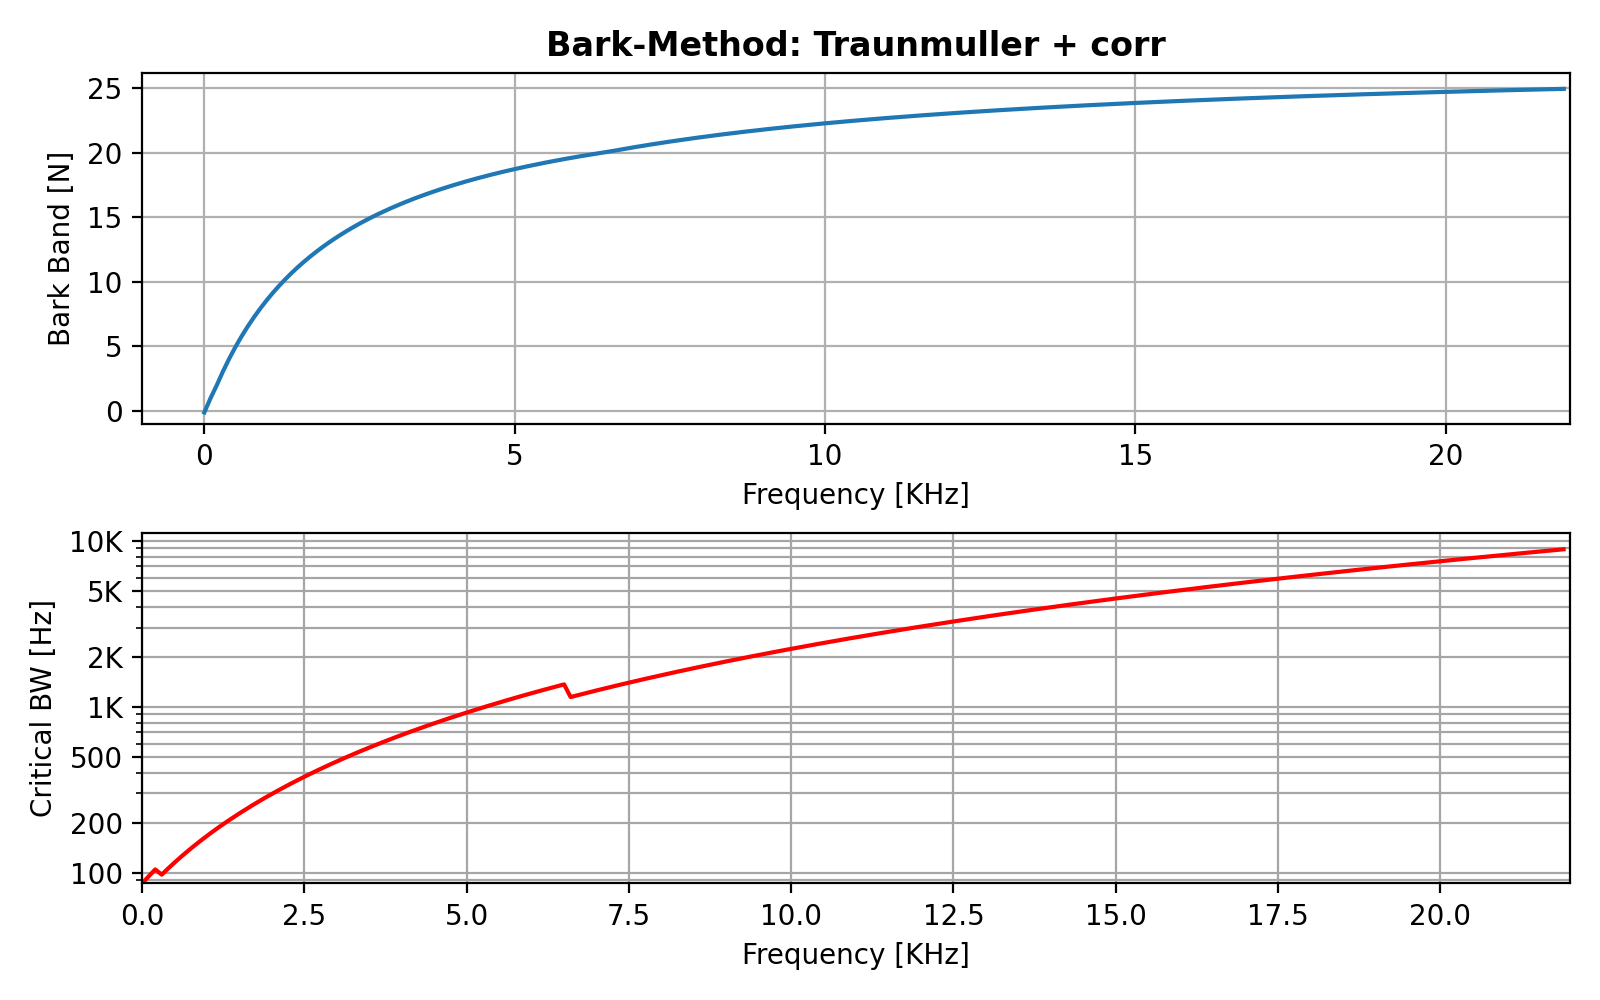
\includegraphics[width=0.75\linewidth]{Experiments/images/Traunmuller_fix}
    \caption{Traunmuller's fixed bark scale and critical bands}\label{fig:Traunmuller_fix}
\end{figure}

The fourth possible modeling equation is proposed by
Schroeder in \cite{SchroederScale} and is as follows:
% Schroeder Eq
\begin{align}
    Bark & = 7\ln \left( \frac{f}{650} + \sqrt{1 + \frac{f^{2}}{422500} }  \right)
\end{align}

Schroeder's bark scale and it's corresponding critical bands
are shown in Figure \ref{fig:Schroeder_bark}
\begin{figure}[H]
    \centering
    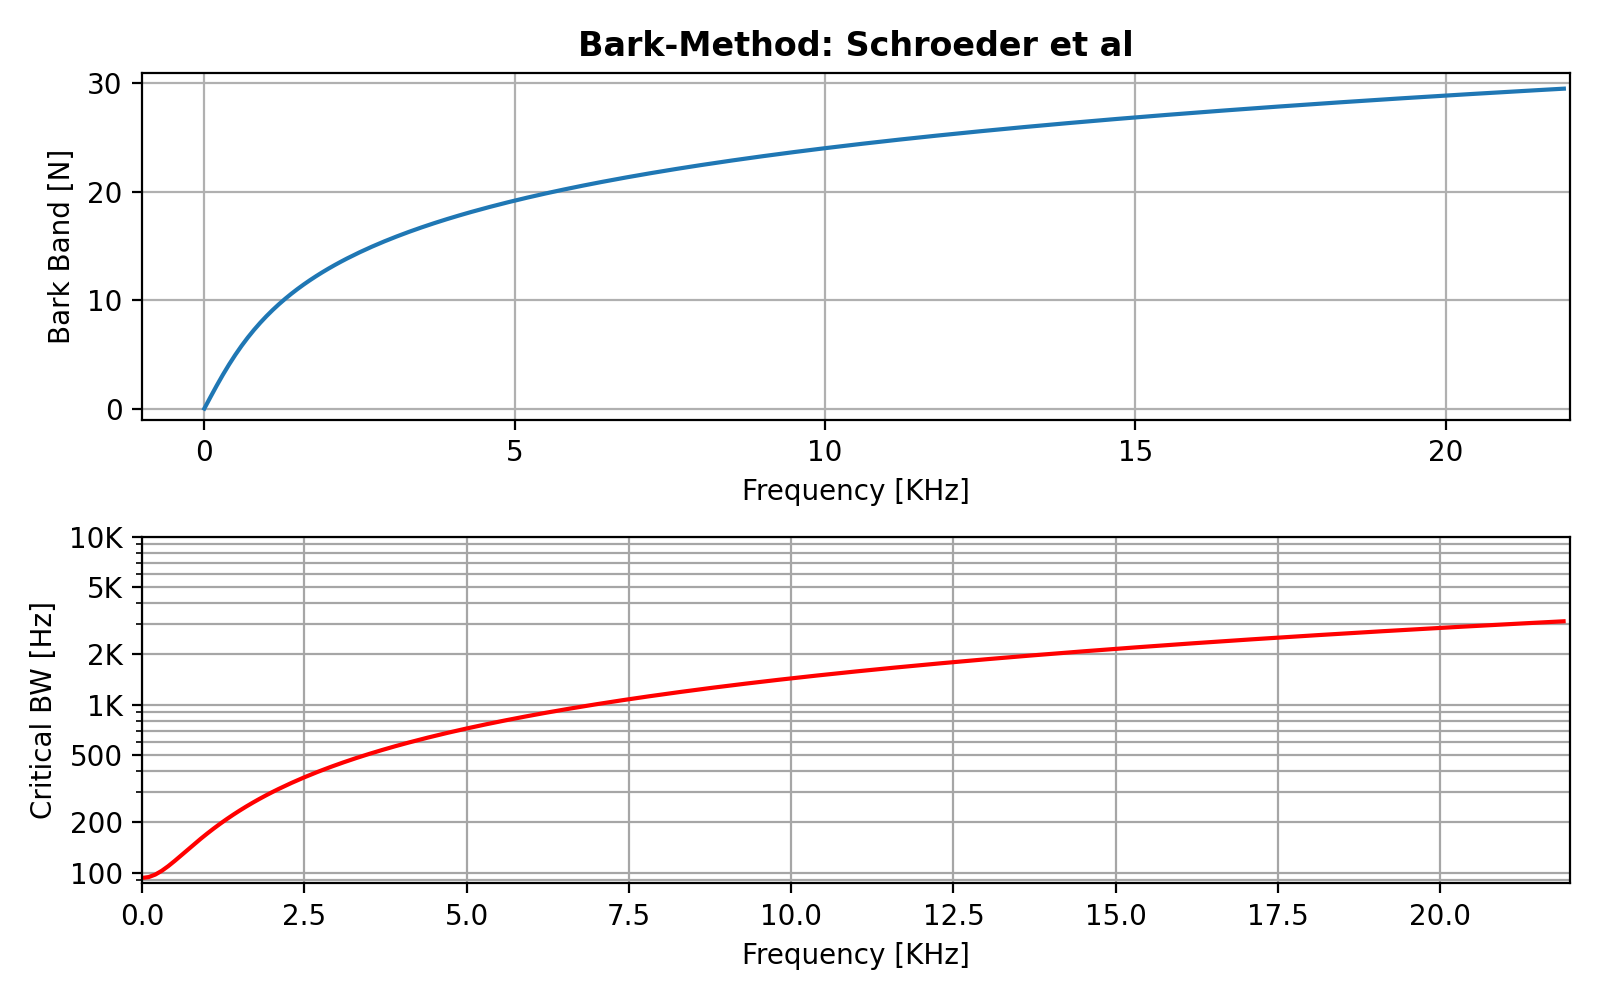
\includegraphics[width=0.75\linewidth]{Experiments/images/Schroeder}
    \caption{Schroeder's bark scale and critical bands}\label{fig:Schroeder_bark}
\end{figure}

% \begin{figure}[H]
%     \centering
%     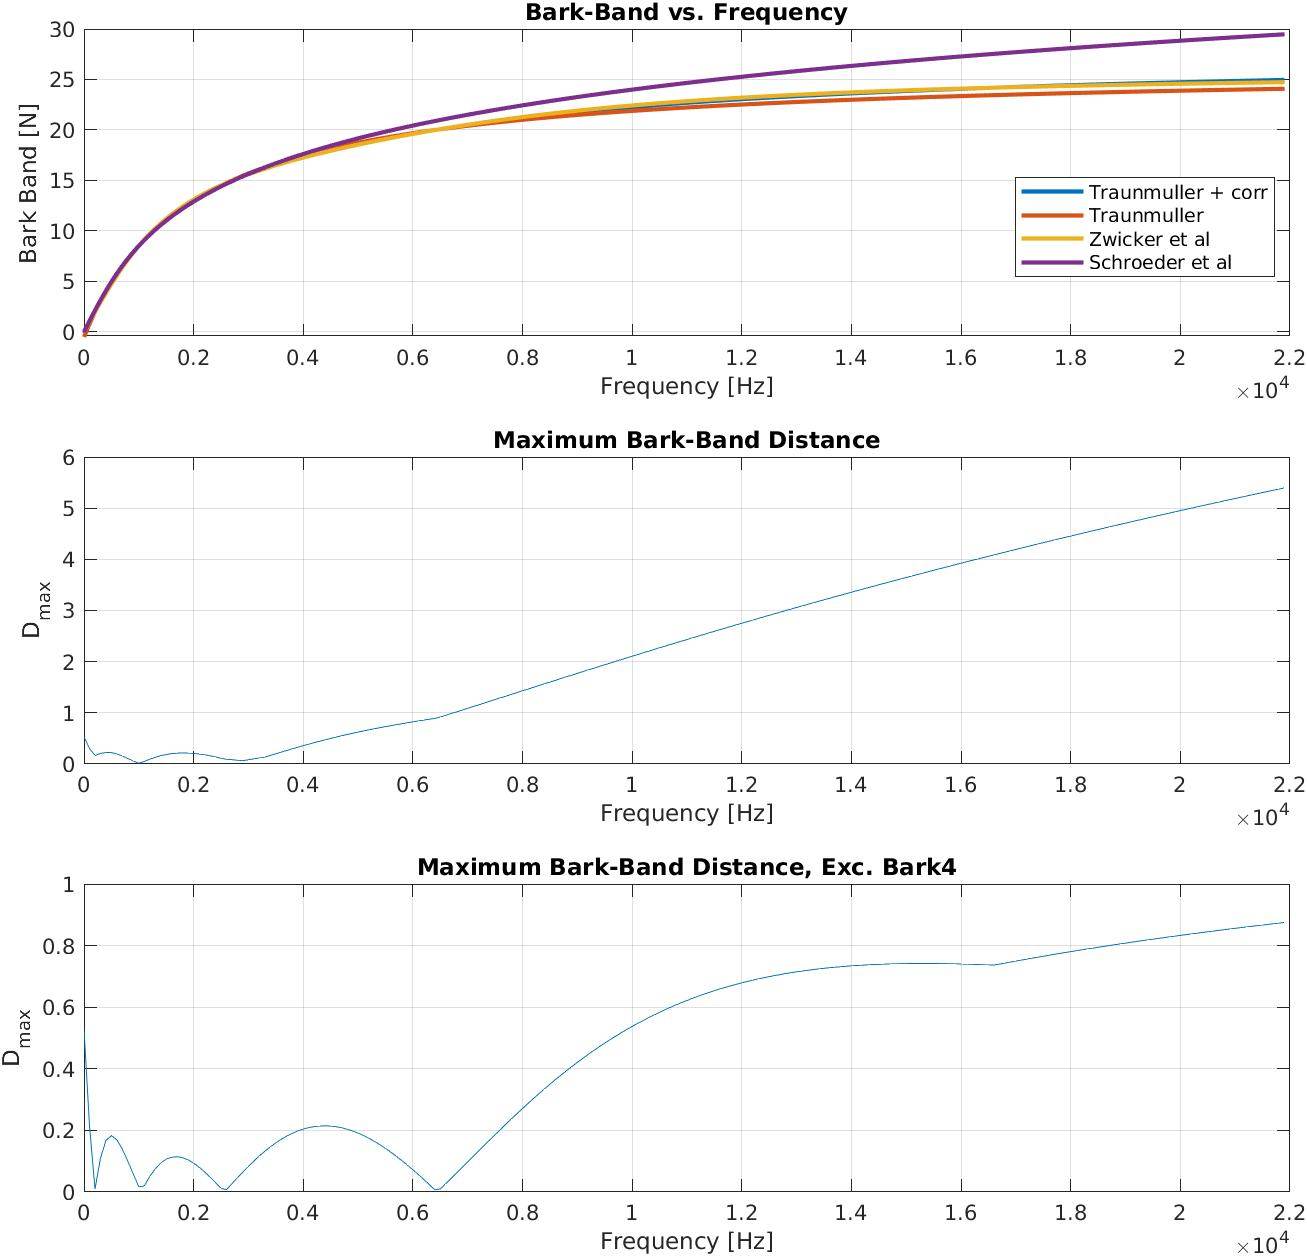
\includegraphics[width=0.75\linewidth]{Experiments/images/bark_comparison}
%     \caption{Bark comparisons}\label{fig:bark_comparison}
% \end{figure}
Figure \ref{fig:bark_comparison} shows a comparison between the four
bark scaling methods.
\begin{figure}[H]
    \centering
    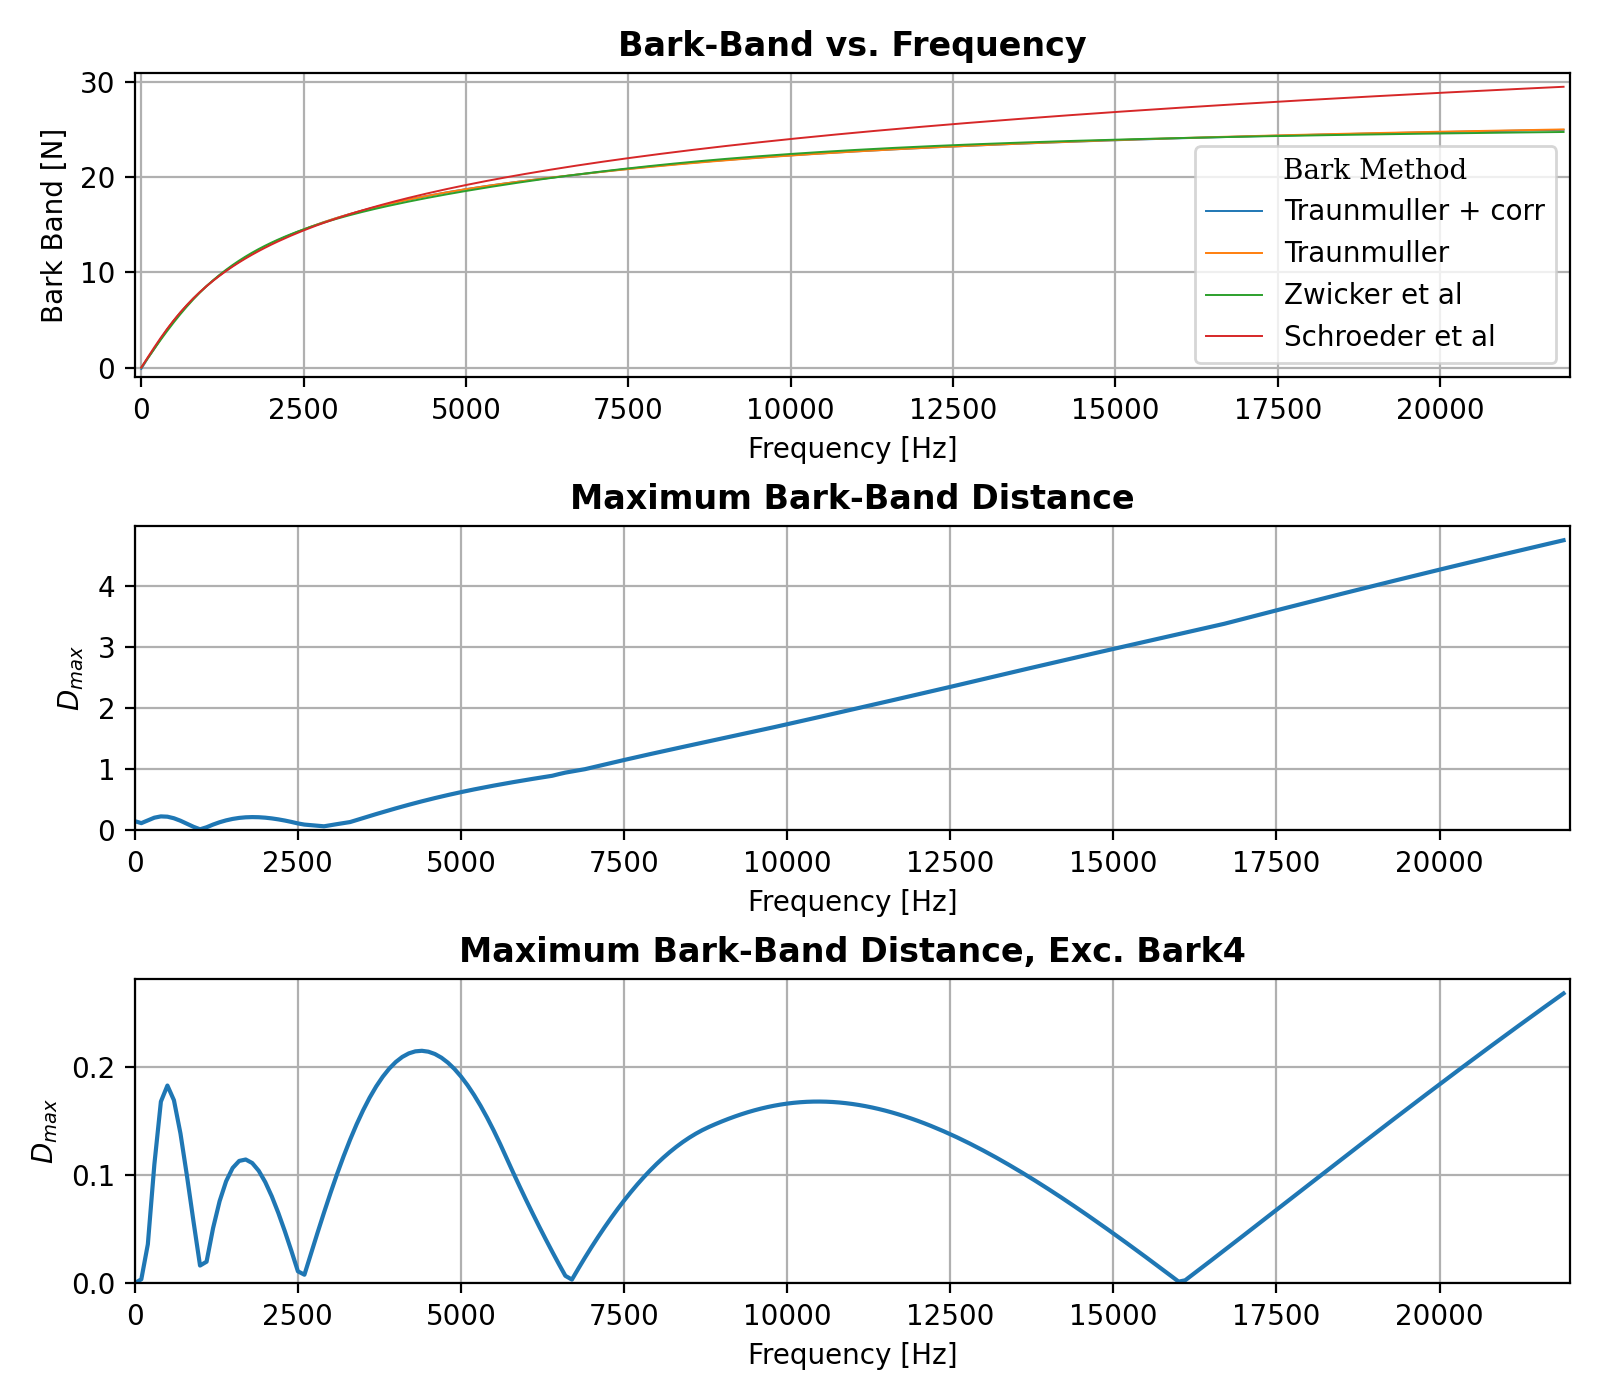
\includegraphics[width=0.95\linewidth]{Experiments/images/bark_comparison2}
    \caption{Bark Scale comparisons}\label{fig:bark_comparison}
\end{figure}

We see in Figure \ref{fig:bark_comparison} that Schroeder's bark scale
has a large error term when compared to the other suggested bark scales.
On the other hand, when we omit Schroeder's scale
and measure the maximum distance between the other threesuggested scales,
we see that the error is comparatively lower. 
% Thus, we deduce that these three are very close in value and just differ
% in their mathimatical expression.

We intend to simplify our implementations in hardware as much as possible.
Simplifications are expressed in utilizing less hardware resources.
This is possible especially when using basic arithmetic operations.
Therefore, we decide to focus on Traunmuller's original bark scale
given in Equation \ref{eq:traunmuller_no_fix}

The accuracy estimation for Traunmuller's original bark scale
is shown in Figure \ref{fig:bark_traunmuller_no_fix}.

\begin{figure}[H]
    \centering
    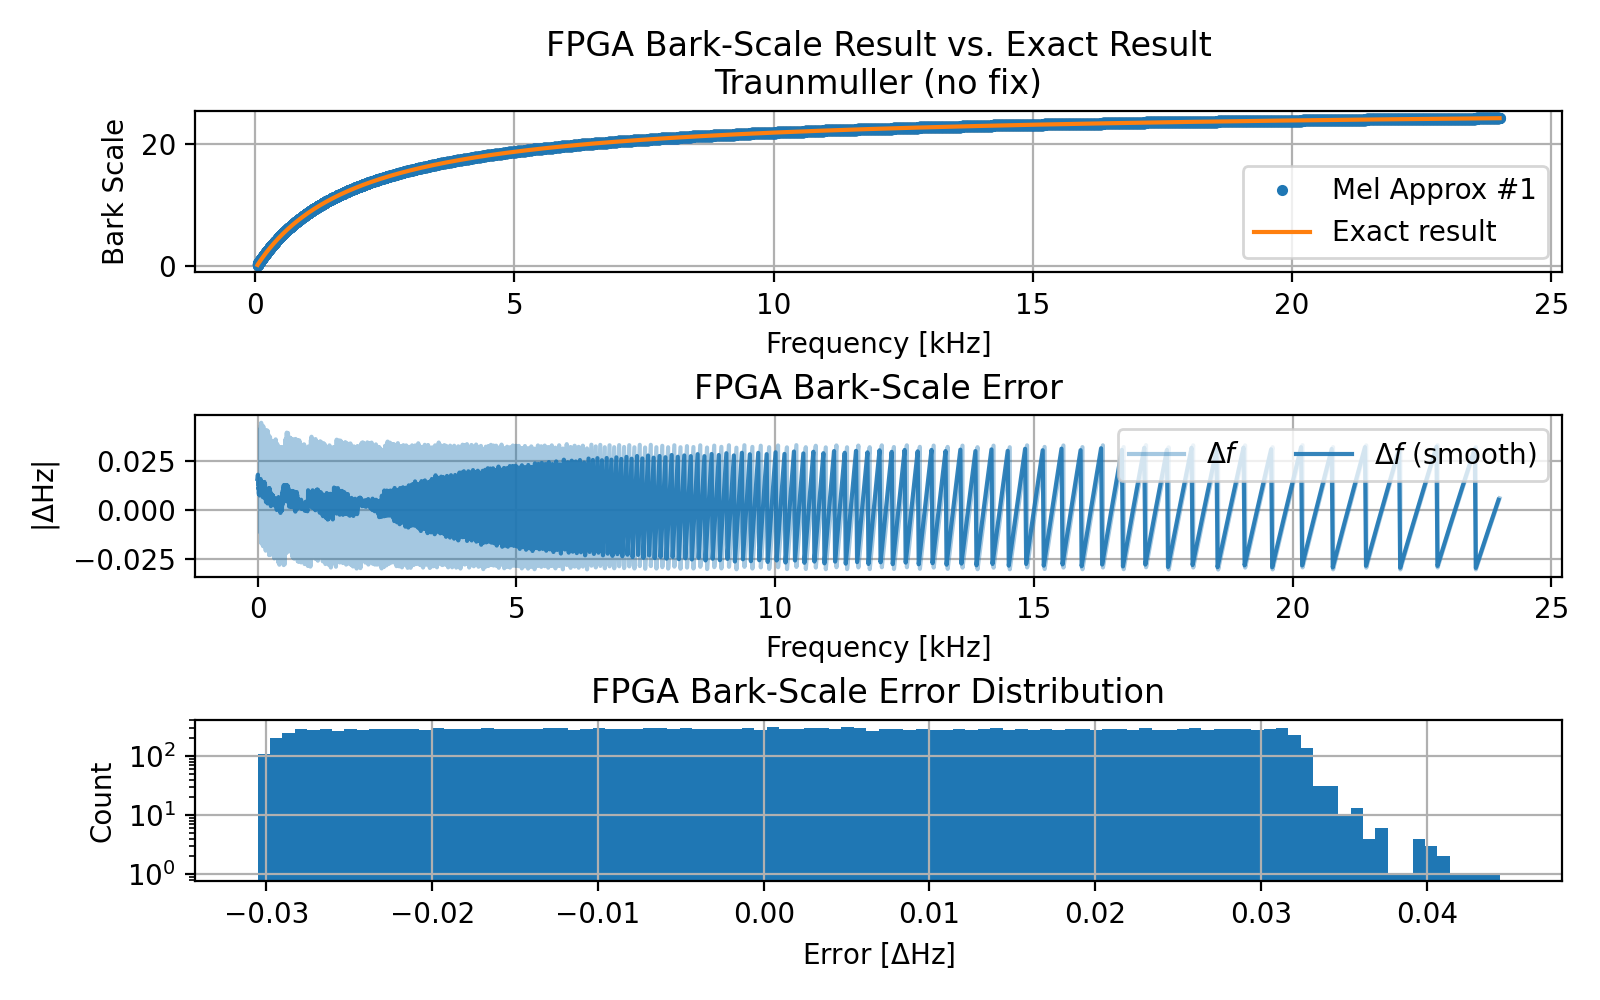
\includegraphics[width=0.95\linewidth]{Scaling/images/bark_traunmuller_no_fix.png}
    \caption{Traunmuller's original bark scale FPGA implementation results}\label{fig:bark_traunmuller_no_fix}
\end{figure}

\begin{table}[H]
    % for more info see: https://www.overleaf.com/learn/latex/tables
    % \centering
    \hspace*{-1.8cm}
    \arrayrulecolor{mtblborder}
\begin{tabular}{ !{\color{mtblborder}\vrule}l!{\color{mtblborder}\vrule}rcccc| } 
    \hline

    \hline
    \rowcolor{mtblcaption} \color{white}\bf{Algorithm} 
    & \color{white}\bf{Latency \([ns]\)}  
    & \color{white}\bf{Quant.} 
    & \color{white}\bf{Max Err. \([\Delta Hz]\)}
    & \color{white}\bf{Mean Err.}
    & \color{white}\bf{Std Err.} \\
    \hline

    \hline
    \rowcolor{mtbl} Traunmuller w/ Fix   & 14 (3 C.C) & U10/5 & N.A & N.A & N.a \\
    \hline
    
    \hline
    \rowcolor{wtbl} Traunmuller w/o Fix  & 9 (2 C.C) &  U9/4  & 0.0443 & 0.0015 & 0.0180 \\
    \hline

    \hline
\end{tabular}
\arrayrulecolor{black}
\caption{Traunmuller's Bark scale implementations performance comparison}
\label{tbl:bark_implementations_performance}
\end{table}


\begin{table}[H]
    % for more info see: https://www.overleaf.com/learn/latex/tables
    \centering
    \arrayrulecolor{ytblborder}
\begin{tabular}{ !{\color{ytblborder}\vrule}l!{\color{ytblborder}\vrule}rrrrr| } 
    \hline

    \hline
    \rowcolor{ytblcaption} \color{white}\bf{Algorithm} 
    & \color{white}\bf{FF} 
    & \color{white}\bf{LUT} 
    & \color{white}\bf{DSP} 
    & \color{white}\bf{LUTRAM} 
    & \color{white}\bf{BRAM} \\
    % & \color{white}\bf{ORM} 
    % & \color{white}\bf{Clean} \\
    \hline

    \hline
    \rowcolor{ytbl} Traunmuller w/ Fix   & 43(0.02\%) & 302(0.26\%) & 1(<1\%) & 0(0\%) & 0(0\%)  \\
    \hline
    
    \hline
    \rowcolor{wtbl} Traunmuller w/o Fix      & 27(0.01\%) & 284(0.24\%) & 1(<1\%) & 0(0\%)  & 0(0\%)    \\
    \hline

    \hline
\end{tabular}
\arrayrulecolor{black}
\caption{Traunmuller's Bark scale implementations resource utilization table}
\label{tbl:Bark_resource_util}
\end{table}


\begin{table}[H]
    % for more info see: https://www.overleaf.com/learn/latex/tables
    \centering
    \arrayrulecolor{gtblborder}
\begin{tabular}{ |l|cc| } 
    \hline

    \hline
    \rowcolor{gtblcaption} \color{white}\bf{Parameter} 
    & \color{white}\bf{Traunmuller w/ Fix} 
    & \color{white}\bf{Traunmuller w/o Fix} \\
    \hline\hline
    \rowcolor{wtbl}\multicolumn{3}{|c|}{\bf{Dynamic Power [W]}}\\
    \hline
    \rowcolor{gtbl} Signals                 & 2.380 & 2.192   \\
    \hline
    
    \hline
    \rowcolor{wtbl} Logic                   & 3.079 & 2.957   \\
    \hline

    \hline
    \rowcolor{gtbl} DSP                     & 1.445 & 0.014  \\
    \hline
    
    \hline
    \rowcolor{wtbl} I/O                     & 4.022 & 4.022  \\
    \hline
    
    \hline
    \rowcolor{gtbl} \(\mathbf{P_{dynmic}}\) & \textbf{10.923} & \textbf{\color{gtblborder}9.186}  \\
    \hline

    % \hline
    % \rowcolor{gtbl} Bark Scale      & 56(0.02\%) & 218(\%) & 1(<1\%)   \\
    % % \cline{2-8}
    % % \multirow{-2}{*}{\cellcolor{ytbl}\#1(5)}   & 14.03/17.78 & 27.06 & 13.73 & - & - & - & 7.72 \\ 
    \hline\hline
    \rowcolor{wtbl}\multicolumn{3}{|c|}{\bf{Static Power [W]}}   \\
    \hline

    \hline
    \rowcolor{gtbl} PL Static               & 0.469 & 0.437  \\
    \hline
    
    \hline
    \rowcolor{wtbl} PS Static               & 0.017 & 0.016   \\
    \hline

    \hline
    \rowcolor{gtbl} \(\mathbf{P_{static}}\) & \textbf{0.486} & \textbf{\color{gtblborder}0.453}   \\
    \hline

    \hline\hline
    \rowcolor{wtbl}\multicolumn{3}{|c|}{\bf{Total Power [W]}}   \\
    \hline

    \hline
    \rowcolor{gtbl} \(\mathbf{P_{total}}\)  & \textbf{11.412} & \textbf{\color{gtblborder}9.639}  \\
    \hline
\end{tabular}
\arrayrulecolor{black}
\caption{Traunmuller's Bark scale implementations Power consumption}
\label{tbl:bark_scale_pwr_tbl}
\end{table}

Table\;\ref{tbl:bark_implementations_performance} summarizes
the performance comparison between the different Bark scaling
implementation approaches. 

Tables\;\ref{tbl:Bark_resource_util} and \ref{tbl:bark_scale_pwr_tbl}
show the synthesis and implementation results 
plus the power estimation reports. 
These reports were taken from the Xilinx Vivado Suite application.

\section{ERB - Equivalent Rectangular Bandwidth}
Like the Bark scaling method, the ERB scale aims 
to rescale the audio spectrum in different 
bandwidths corresponding to the human hearing ``filters''.

This approach slightly differs from the Bark scale
because the filter is modeled according
to a rectangular filter with an equivalent
bandwidth.
\begin{align}\label{eq:erb_eq}
    ERBs = 11.17\ln (47.065 - \frac{676170.42}{f + 14678.5})    
\end{align}

A proposed approximation is given by:
\begin{align}\label{eq:erb_approx_eq}
    ERBs = 21.4 \cdot \log_{10} (1 + 0.00437f)    
\end{align}


% \subsection{ERB Critical Bands}
The accuracy estimation for the LUT based ERB scale
and the LUT based ERB approximation are shown in Figures 
\ref{fig:erb_fpga}, \ref{fig:erb_approx} respectively.

\begin{figure}[H]
    \centering
    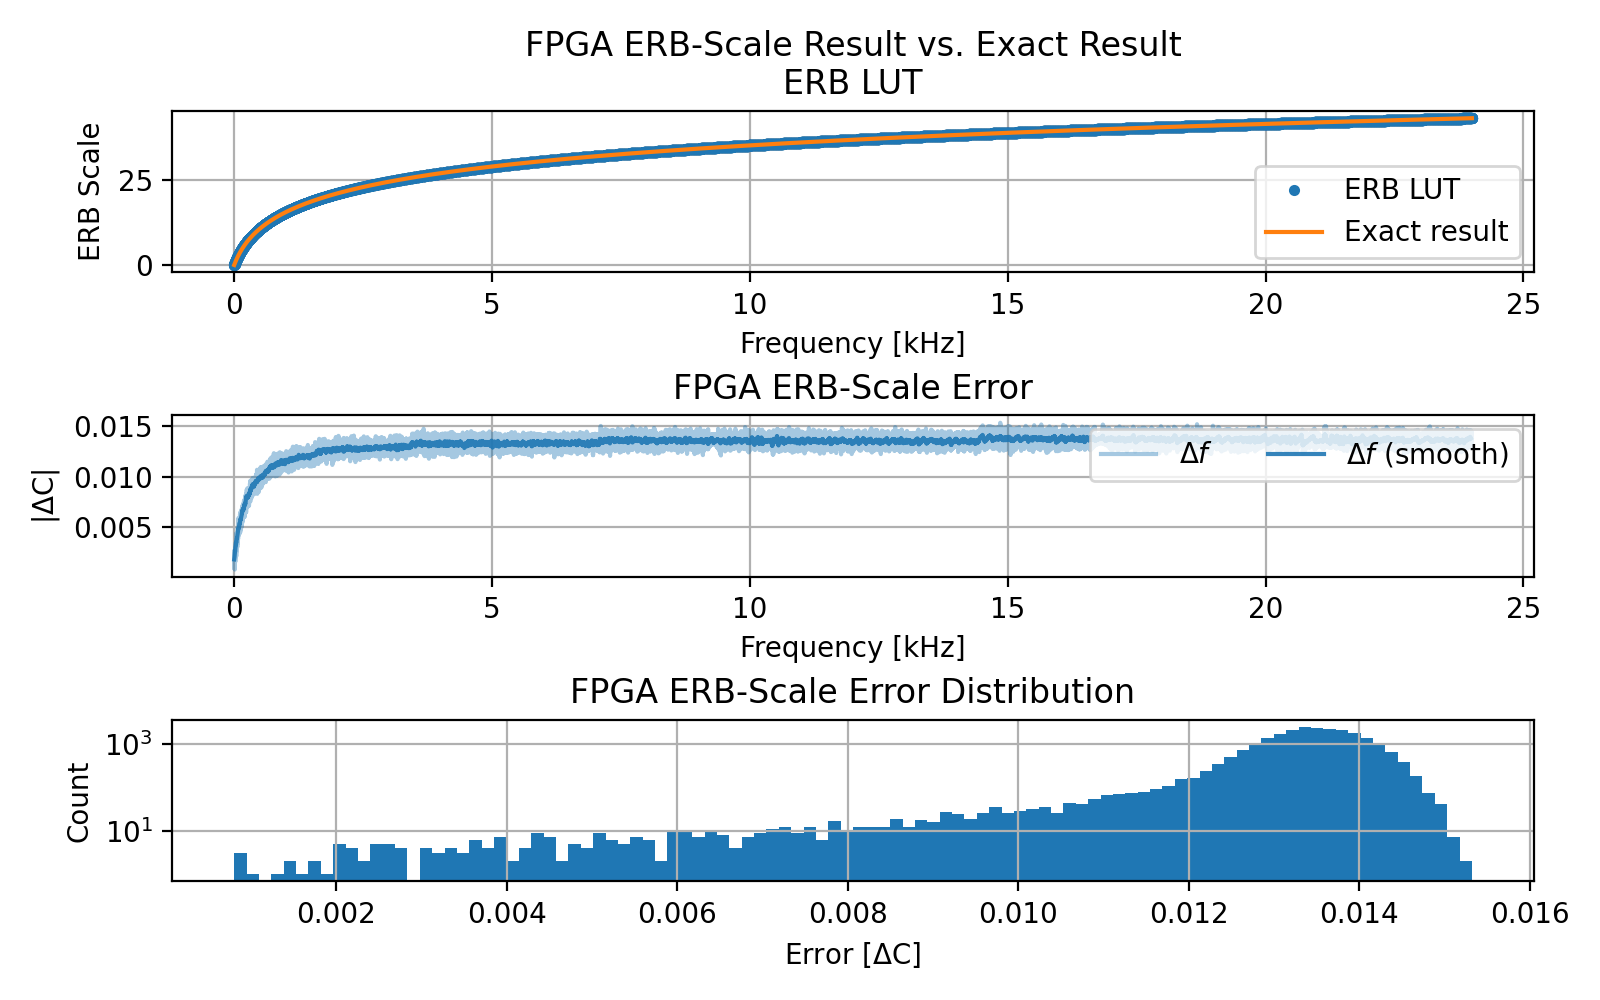
\includegraphics[width=0.75\linewidth]{Scaling/images/erb}
    \caption{LUT based ERB FPGA implementation results}\label{fig:erb_fpga}
\end{figure}

\begin{figure}[H]
    \centering
    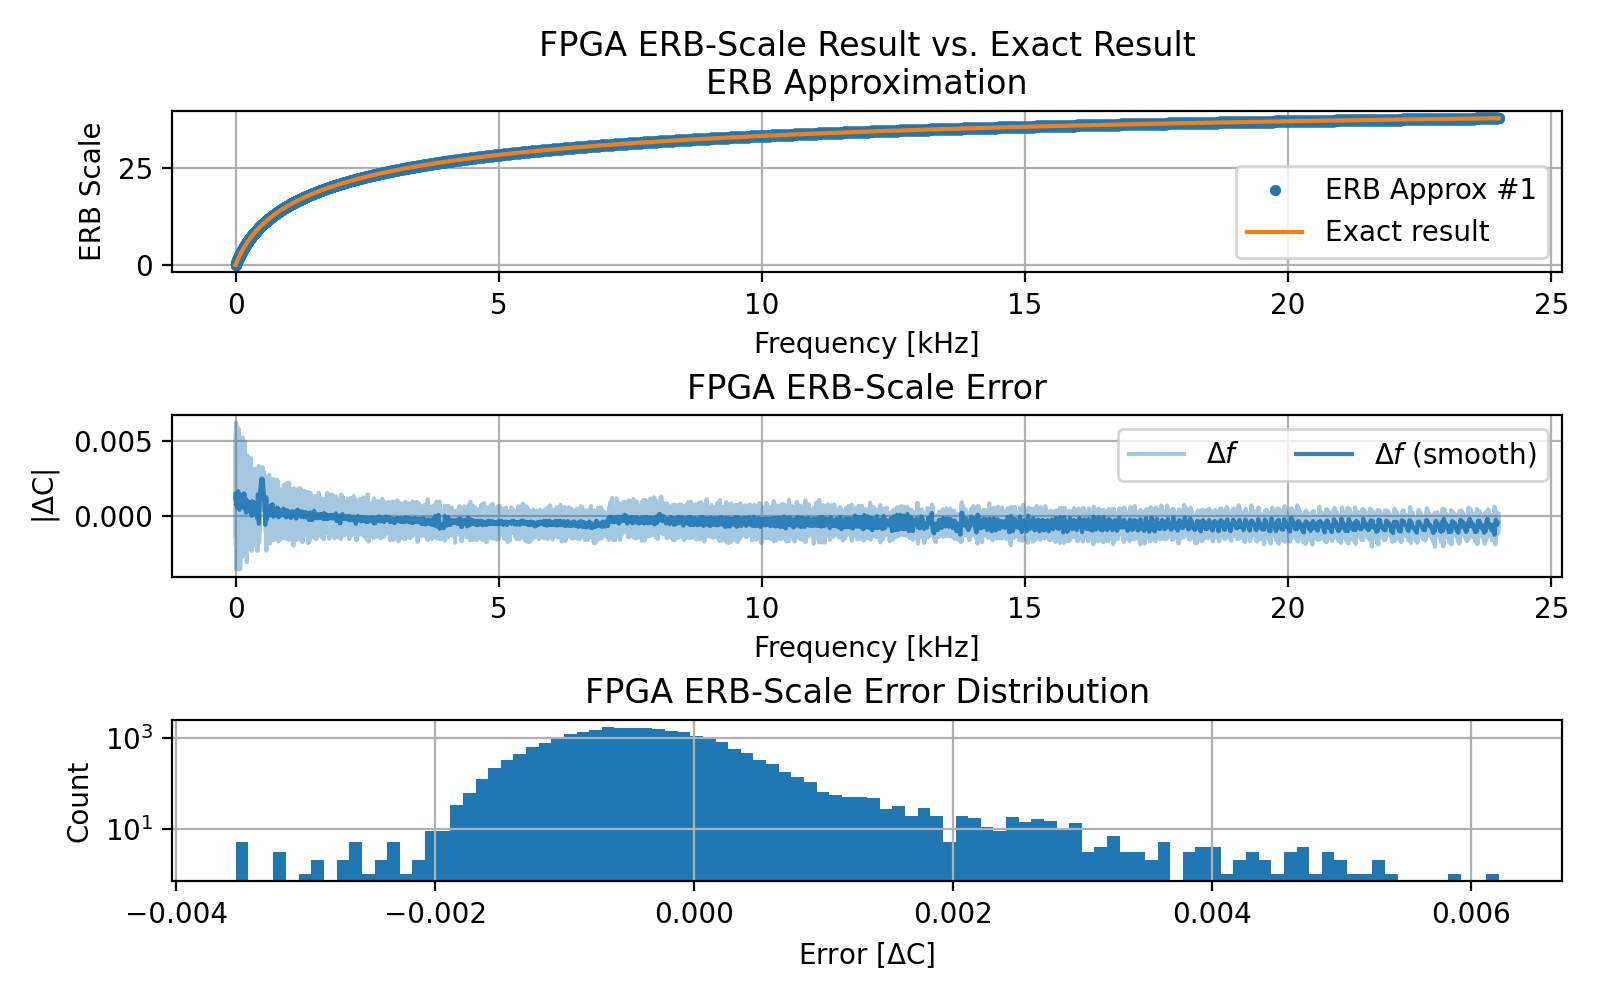
\includegraphics[width=0.75\linewidth]{Scaling/images/erb_approx}
    \caption{LUT based ERB approximation FPGA implementation results}\label{fig:erb_approx}
\end{figure}


\begin{table}[H]
    % for more info see: https://www.overleaf.com/learn/latex/tables
    \centering
    % \hspace*{-1.8cm}
    \arrayrulecolor{mtblborder}
\begin{tabular}{ !{\color{mtblborder}\vrule}l!{\color{mtblborder}\vrule}rcccc| } 
    \hline

    \hline
    \rowcolor{mtblcaption} \color{white}\bf{Algorithm} 
    & \color{white}\bf{Latency \([ns]\)}  
    & \color{white}\bf{Quant.} 
    & \color{white}\bf{Max Err. \([\Delta C]\)}
    & \color{white}\bf{Mean Err.}
    & \color{white}\bf{Std Err.} \\
    \hline

    \hline
    \rowcolor{mtbl} ERB   & 23 (5 C.C) & U16/10 & 0.0153 & 0.0130 & 0.0018 \\
    \hline
    
    \hline
    \rowcolor{wtbl} ERB Approx  & 14 (3 C.C) &  U16/10  & 6.210m & -0.408m & 0.657m \\
    \hline

    \hline
\end{tabular}
\arrayrulecolor{black}
\caption{ERB and ERB approx performance comparison}
\label{tbl:erb_scale_performance}
\end{table}

Table\;\ref{tbl:erb_scale_performance} presents the performance
comparison between the implementations of the pure ERB
and the ERB approximation
given by Equations\;\ref{eq:erb_eq} 
and \ref{eq:erb_approx_eq}, respectively. The error terms
for the ERBs are measured in \(\Delta C\), indicating the
error in Cams rather than in frequency units (Hz). 
Equation\;\ref{eq:cams_hz} can be used to convert Cams to Hz.
\begin{align}\label{eq:cams_hz}
    f = \frac{676170.42}{47.065 - e^{0.0895\cdot C}} - 14678.5
\end{align}

\begin{table}[H]
    % for more info see: https://www.overleaf.com/learn/latex/tables
    \centering
    \arrayrulecolor{ytblborder}
\begin{tabular}{ !{\color{ytblborder}\vrule}l!{\color{ytblborder}\vrule}rrrrr| } 
    \hline

    \hline
    \rowcolor{ytblcaption} \color{white}\bf{Algorithm} 
    & \color{white}\bf{FF} 
    & \color{white}\bf{LUT} 
    & \color{white}\bf{DSP} 
    & \color{white}\bf{LUTRAM} 
    & \color{white}\bf{BRAM} \\
    % & \color{white}\bf{ORM} 
    % & \color{white}\bf{Clean} \\
    \hline

    \hline
    \rowcolor{ytbl} ERB   & 112(0.05\%) & 824(0.70\%) & 1(<1\%) & 1(0.02\%) & 1.5(1.04\%)  \\
    \hline
    
    \hline
    \rowcolor{wtbl} ERB Approx      & 103(0.04\%) & 564(0.48\%) & 1(<1\%) & 1(0.01\%)  & 1.5(1.04\%)    \\
    \hline

    \hline
\end{tabular}
\arrayrulecolor{black}
\caption{ERB scaling methods resource utilization table}
\label{tbl:ERB_resource_util}
\end{table}


\begin{table}[H]
    % for more info see: https://www.overleaf.com/learn/latex/tables
    \centering
    \arrayrulecolor{gtblborder}
\begin{tabular}{ |l|cc| } 
    \hline

    \hline
    \rowcolor{gtblcaption} \color{white}\bf{Parameter} 
    & \color{white}\bf{ERB} 
    & \color{white}\bf{ERB Approx} \\
    \hline\hline
    \rowcolor{wtbl}\multicolumn{3}{|c|}{\bf{Dynamic Power [W]}}\\
    \hline
    \rowcolor{gtbl} Signals                 & 12.691 & 5.525   \\
    \hline
    
    \hline
    \rowcolor{wtbl} Logic                   & 17.576 & 7.478   \\
    \hline

    \hline
    \rowcolor{gtbl} DSP                     & 0.067 & 0.049  \\
    \hline
    
    \hline
    \rowcolor{wtbl} I/O                     & 17.379 & 17.373  \\
    \hline
    
    \hline
    \rowcolor{gtbl} \(\mathbf{P_{dynmic}}\) & \textbf{47.713} & \textbf{\color{gtblborder}31.519}  \\
    \hline

    % \hline
    % \rowcolor{gtbl} Bark Scale      & 56(0.02\%) & 218(\%) & 1(<1\%)   \\
    % % \cline{2-8}
    % % \multirow{-2}{*}{\cellcolor{ytbl}\#1(5)}   & 14.03/17.78 & 27.06 & 13.73 & - & - & - & 7.72 \\ 
    \hline\hline
    \rowcolor{wtbl}\multicolumn{3}{|c|}{\bf{Static Power [W]}}   \\
    \hline

    \hline
    \rowcolor{gtbl} PL Static               & 2.971 & 1.510  \\
    \hline
    
    \hline
    \rowcolor{wtbl} PS Static               & 0.084 & 0.046   \\
    \hline

    \hline
    \rowcolor{gtbl} \(\mathbf{P_{static}}\) & \textbf{3.055} & \textbf{\color{gtblborder}1.556}   \\
    \hline

    \hline\hline
    \rowcolor{wtbl}\multicolumn{3}{|c|}{\bf{Total Power [W]}}   \\
    \hline

    \hline
    \rowcolor{gtbl} \(\mathbf{P_{total}}\)  & \textbf{50.768} & \textbf{\color{gtblborder}33.075}  \\
    \hline
\end{tabular}
\arrayrulecolor{black}
\caption{ERB vs. ERB approx Power consumption}
\label{tbl:erb_scale_pwr_tbl}
\end{table}

Tables\;\ref{tbl:ERB_resource_util} and \ref{tbl:erb_scale_pwr_tbl}
show the synthesis and implementation results 
plus the power estimation reports for the ERB implementations. 


% \begin{table}[H]
%     % for more info see: https://www.overleaf.com/learn/latex/tables
%     \centering
%     \begin{tabular}{|c|r|r|r|r|r|}
%       \hline
%       $N$ & Latency ($\mu s$) & FF & LUT & DSP48 & BRAM \\
%       \hline
%         3  & 4.80  &   3889 (27.6\%)                 &    3901 (54.9\%)                  &   90 (25.0\%) & 0 (0.0\%) \\
%         4  & 6.34  &  63657 (45.1\%)                 &   64149 (90.4\%)                  &  144 (40.0\%) & 0 (0.0\%) \\
%         8  & 12.50 & 231199 (\textcolor{red}{164\%}) &  252446 (\textcolor{red}{356\%})  &  272 (75.6\%) & 0 (0.0\%) \\
%         16 & 24.82 & 895377 (\textcolor{red}{635\%}) & 1040992 (\textcolor{red}{1466\%}) &  144 (40.0\%) & 0 (0.0\%) \\
%        \hline
%     \end{tabular}
%     \caption{\bf{ IQRD Performance:} Latency, Resource Utilization, and Power for \(log_{10}\) LUT on FPGA}
%     \label{tbl:IQRD_perf}
% \end{table}

\section{Summary}

The following tables\;\ref{tbl:IQRD_perf}, 
\;\ref{tbl:scale_performance_tbl} and \;\ref{tbl:sum_scale_pwr_tbl},
provide a summary of the
resource utilization, timing and accuracy performances, and lastly 
the power consumption of each scaling implementation.

\begin{table}[H]
    % for more info see: https://www.overleaf.com/learn/latex/tables
    \centering
    \arrayrulecolor{ytblborder}
\begin{tabular}{ !{\color{ytblborder}\vrule}l!{\color{ytblborder}\vrule}rrrrr| } 
    \hline

    \hline
    \rowcolor{ytblcaption} \color{white}\bf{Algorithm} 
    & \color{white}\bf{FF} 
    & \color{white}\bf{LUT} 
    & \color{white}\bf{DSP} 
    & \color{white}\bf{LUTRAM} 
    & \color{white}\bf{BRAM} \\
    % & \color{white}\bf{ORM} 
    % & \color{white}\bf{Clean} \\
    \hline

    \hline
    \rowcolor{ytbl} Log-Based Mel   & 82(0.04\%) & 276(0.23\%) & 1(<1\%) & 10(0.02\%) & 1.5(1.04\%) \\
    \hline
    
    \hline
    \rowcolor{wtbl} Mel \#1 Generic     & 47(0.02\%) & 269(0.19\%) & 1(<1\%) & 0(0\%)  & 0(0\%)    \\
    \hline
    
    \hline
    \rowcolor{ytbl} Bark Scale w/ fix     & 43(0.02\%) & 302(0.26\%) & 1(<1\%) & 0(0\%) & 0(0\%)  \\
    \hline

    \hline
    \rowcolor{wtbl} Bark Scale w/o fix     & 27(0.01\%) & 284(0.24\%) & 1(<1\%) & 0(0\%)  & 0(0\%)    \\
    \hline

    \hline
    \rowcolor{ytbl} Approx. ERB     & 103(0.04\%) & 564(0.48\%) & 1(<1\%) & 1(0.01\%)  & 1.5(1.04\%)    \\
    \hline

    \hline
\end{tabular}
\arrayrulecolor{black}
\caption{Mel-Approx, log-based Mel, Bark Scale, and approximated ERB resources utilization comparison}
\label{tbl:IQRD_perf}
\end{table}





% \begin{table}[H]
%     % for more info see: https://www.overleaf.com/learn/latex/tables
%     \centering
%     \arrayrulecolor{gtblborder}
% \begin{tabular}{ !{\color{gtblborder}\vrule}l!{\color{gtblborder}\vrule}rrrrrr| } 
%     \hline

%     \hline
%     \rowcolor{gtblcaption} \color{white}\bf{Algorithm} 
%     & \color{white}\bf{Signals} 
%     & \color{white}\bf{Logic} 
%     & \color{white}\bf{DSP} 
%     & \color{white}\bf{IO} 
%     & \color{white}\bf{BRAM}
%     & \color{white}\bf{Total} \\
%     \hline

%     \hline
%     \rowcolor{gtbl} Log Based Mel   & 82(0.04\%) & 276(\%) & 1(<1\%) & 18 & 1.5 & 0 \\
%     \hline
    
%     \hline
%     \rowcolor{wtbl} Approx. Mel     & 47(0.02\%) & 230(\%) & 1(<1\%) & 0  & 0   & 0 \\
%     \hline
    
%     \hline
%     \rowcolor{gtbl} Bark Scale      & 56(0.02\%) & 218(\%) & 1(<1\%) & 0  & 0   & 0 \\
%     % \cline{2-8}
%     % \multirow{-2}{*}{\cellcolor{ytbl}\#1(5)}   & 14.03/17.78 & 27.06 & 13.73 & - & - & - & 7.72 \\ 
%     \hline

%     \hline
% \end{tabular}
% \arrayrulecolor{black}
% \caption{Mel-Approx, log based Mel, Bark Scale Power consumption}
% \label{tbl:scale_pwr_tbl}
% \end{table}


\begin{table}[H]
    % for more info see: https://www.overleaf.com/learn/latex/tables
    % \centering
    \hspace*{-1.8cm}
    \arrayrulecolor{mtblborder}
\begin{tabular}{ !{\color{mtblborder}\vrule}l!{\color{mtblborder}\vrule}rcccc| } 
    \hline

    \hline
    \rowcolor{mtblcaption} \color{white}\bf{Algorithm} 
    & \color{white}\bf{Latency \([ns]\)}  
    & \color{white}\bf{Quant.} 
    & \color{white}\bf{Max Err. \([\Delta Hz]\)}
    & \color{white}\bf{Mean Err.}
    & \color{white}\bf{Std Err.} \\
    \hline

    \hline
    \rowcolor{mtbl} Log-Based Mel   & 14 (3 C.C) & U16/4 & 1.146 & 0.268 & 0.106 \\
    \hline
    
    \hline
    \rowcolor{wtbl} Mel \#1 Generic     & 9 (2 C.C) &  U16/4  & 0.174 & -0.035 & 0.061 \\
    \hline
    
    \hline
    \rowcolor{mtbl} Bark Scale w/ fix      & 14 (3 C.C) &  U10/5 & N.A & N.A & N.A \\
    % \cline{2-8}
    % \multirow{-2}{*}{\cellcolor{ytbl}\#1(5)}   & 14.03/17.78 & 27.06 & 13.73 & - & - & - & 7.72 \\ 
    \hline

    \hline
    \rowcolor{wtbl} Bark Scale w/o fix     & 9 (2 C.C) &  U9/4  & 0.0443 & 1.5m & 0.0015 \\
    \hline

    \hline
    \rowcolor{mtbl} ERB Approx.     & 14 (3 C.C) &  U16/10  & 0.292 & 0.104 & 0.134 \\
    \hline

    \hline
\end{tabular}
\arrayrulecolor{black}
\caption{Mel-Approx, log-based Mel, Bark Scale performance comparison}
\label{tbl:scale_performance_tbl}
\end{table}


\begin{table}[H]
    % for more info see: https://www.overleaf.com/learn/latex/tables
    % \centering
    \hspace*{-1cm}
    \arrayrulecolor{gtblborder}
\begin{tabular}{ |l|ccccc| } 
    \hline

    \hline
    \rowcolor{gtblcaption} \color{white}\bf{Parameter} 
    & \color{white}\bf{Mel LUT}
    & \color{white}\bf{Mel Gen}
    & \color{white}\bf{Bark w/}
    & \color{white}\bf{Bark w/o}
    & \color{white}\bf{Approx. ERB} \\
    \hline\hline
    \rowcolor{wtbl}\multicolumn{6}{|c|}{\bf{Dynamic Power [W]}}\\
    \hline
    \rowcolor{gtbl} Signals & 4.947 & 2.916 & 2.380 & 2.192 & 5.525  \\
    \hline
    
    \hline
    \rowcolor{wtbl} Logic & 6.50 & 3.070 & 3.079 & 2.957 & 7.478  \\
    \hline

    \hline
    \rowcolor{gtbl} DSP & 0.014 & 0.014 & 1.445 & 0.014 & 0.049  \\
    \hline
    
    \hline
    \rowcolor{wtbl} I/O & 18.236 & 6.378 & 4.022 & 4.022 & 17.373  \\
    \hline
    
    \hline
    \rowcolor{gtbl} \(\mathbf{P_{dynmic}}\) & \textbf{29.697} & \textbf{12.379} & \textbf{10.923} & \textbf{9.186} & \textbf{31.519}  \\
    \hline

    % \hline
    % \rowcolor{gtbl} Bark Scale      & 56(0.02\%) & 218(\%) & 1(<1\%)   \\
    % % \cline{2-8}
    % % \multirow{-2}{*}{\cellcolor{ytbl}\#1(5)}   & 14.03/17.78 & 27.06 & 13.73 & - & - & - & 7.72 \\ 
    \hline\hline
    \rowcolor{wtbl}\multicolumn{6}{|c|}{\bf{Static Power [W]}}   \\
    \hline

    \hline
    \rowcolor{gtbl} PL Static               & 2.364 & 0.499 & 0.469 & 0.437 & 1.510  \\
    \hline
    
    \hline
    \rowcolor{wtbl} PS Static               & 0.068 & 0.018 & 0.017 & 0.016 & 0.046  \\
    \hline

    \hline
    \rowcolor{gtbl} \(\mathbf{P_{static}}\) & \textbf{2.432} & \textbf{0.517} & \textbf{0.486} & \textbf{0.453} & \textbf{1.556}  \\
    \hline

    \hline\hline
    \rowcolor{wtbl}\multicolumn{6}{|c|}{\bf{Total Power [W]}}   \\
    \hline

    \hline
    \rowcolor{gtbl} \(\mathbf{P_{total}}\)  & \textbf{32.13} & \textbf{12.896} & \textbf{11.412} & \textbf{9.639} & \textbf{33.075}  \\
    \hline
\end{tabular}
\arrayrulecolor{black}
\caption{Mel-Approx, log-based Mel, Bark Scale, and approximated ERB Power consumption}
\label{tbl:sum_scale_pwr_tbl}
\end{table}
\vspace{-0.8cm}
We see that the implementations of the 
approximated Mel scale generic and
the Traunmuller's bark scaling approaches 
were synthesized to the smallest amount of
physical hardware resources. This also supports
the measured power consumptions we see in
Table\;\ref{tbl:sum_scale_pwr_tbl}, where
these scaling implementations 
proved to be the most efficient.

Based on these results, we conducted the research using
these most prominent implementations in the feature extraction modules
and the ASR engine's internal acoustic scaling.